\documentclass[12pt]{article}
\usepackage[utf8]{inputenc}
\usepackage[spanish]{babel}
\spanishdecimal{.}
\usepackage{amsmath, amssymb}
\usepackage{array}
\usepackage{booktabs}
\usepackage{multirow}
\usepackage{graphicx}
\usepackage{grffile}
\usepackage{float}
\usepackage{geometry}
\usepackage{caption}
\usepackage{listings}
\usepackage{xcolor}
\geometry{margin=2.5cm}

\lstset{
  basicstyle=\ttfamily\footnotesize,
  breaklines=true,
  breakatwhitespace=false,
  columns=flexible,
  keepspaces=true,
  showstringspaces=false,
  frame=single,
  framesep=4pt,
  xleftmargin=8pt,
  xrightmargin=4pt,
  backgroundcolor=\color{gray!8},
  commentstyle=\color{gray!55},
  keywordstyle=\bfseries,
  extendedchars=true,
  literate=
    {á}{{\'{a}}}1 {é}{{\'{e}}}1 {í}{{\'{i}}}1 {ó}{{\'{o}}}1 {ú}{{\'{u}}}1
    {Á}{{\'{A}}}1 {É}{{\'{E}}}1 {Í}{{\'{I}}}1 {Ó}{{\'{O}}}1 {Ú}{{\'{U}}}1
    {ñ}{{\~{n}}}1 {Ñ}{{\~{N}}}1 {ü}{{\"u}}1 {Ü}{{\"U}}1
    {¿}{{?`}}1 {¡}{{!`}}1
    {—}{{---}}1
    {–}{{--}}1
    {µ}{{\ensuremath{\mu}}}1
    {°}{{\ensuremath{^\circ}}}1
    {³}{{\textsuperscript{3}}}1
    {²}{{\textsuperscript{2}}}1
    {→}{{->}}1
    {←}{{<-}}1,
}

\title{Proyecto Final --- Regresi\'on Avanzada\\[6pt]
       \large An\'alisis Bayesiano Espacial de PM2.5 en el Valle de M\'exico}
\author{Paulina Garza Allende \and Andrea Monserrat Arredondo Rodr\'iguez \and Othoniel Reyes Camacho}
\date{19 de mayo de 2026}

\begin{document}
\maketitle

\tableofcontents
\bigskip

%==============================================================
\section{Introducci\'on}
%==============================================================

El Valle de M\'exico es una cuenca hidrol\'ogica cerrada que alberga la
Zona Metropolitana del Valle de M\'exico (ZMVM), con aproximadamente
22~millones de habitantes.
Su geometr\'ia de cuenca cerrada impide la ventilaci\'on natural de los
contaminantes, lo que convierte al PM2.5 (material particulado fino con
di\'ametro aerodin\'amico $\leq 2.5\,\mu$m) en uno de los principales
problemas de salud p\'ublica de la regi\'on.
La exposici\'on cr\'onica a PM2.5 est\'a asociada con enfermedades
respiratorias, cardiovasculares y aumento en la mortalidad.

La fuente de datos es el Sistema Nacional de Informaci\'on de la
Calidad del Aire~(SINAICA), operado por el Instituto Nacional de
Ecolog\'ia y Cambio Clim\'atico (INECC, s.f.).
Se descargaron datos de las 56 estaciones de monitoreo ubicadas dentro
de los l\'imites del Valle de M\'exico (16~alcald\'ias de la CDMX,
59~municipios del Estado de M\'exico, m\'as Tizayuca en Hidalgo).
De estas, solo 14~estaciones reportaron simult\'aneamente concentraci\'on
de PM2.5, temperatura y humedad relativa durante 2023,
con un total de 2{,}617~observaciones diarias (enero--diciembre de 2023).

La pregunta central de este proyecto es:
\begin{quote}
\emph{¿Qu\'e tan importante es la estructura espacial para explicar la variaci\'on
de PM2.5 en el Valle de M\'exico, y podemos usarla para predecir la
contaminaci\'on en zonas sin sensores?}
\end{quote}

Para responderla se ajustan seis modelos bayesianos de complejidad
creciente en JAGS a trav\'es del paquete \texttt{R2jags} (Plummer, 2003; R Core Team, 2025):

\begin{enumerate}
  \item \textbf{Modelo A --- Normal global}: ¿cu\'anto de la variaci\'on de PM2.5
        explican el clima y la estacionalidad, sin considerar la ubicaci\'on?
  \item \textbf{Modelo B --- Efectos fijos}: ¿existen diferencias sistem\'aticas
        entre estaciones que no se explican por clima?
  \item \textbf{Modelo C1 --- Jer\'arquico}: ¿es mejor modelar esas diferencias
        como un proceso aleatorio com\'un con encogimiento~(\emph{shrinkage})
        que como par\'ametros independientes?
  \item \textbf{Modelo C2 --- Gamma}: ¿es la distribuci\'on Gamma, que respeta
        el soporte positivo de PM2.5, mejor que la Normal sobre el logaritmo?
  \item \textbf{Modelo D --- Tendencia lat/lon}: ¿captura un gradiente lineal
        en latitud y longitud el patr\'on espacial, o se necesita un modelo
        no lineal?
\end{enumerate}

El \textbf{Modelo E} usa los efectos espaciales del Modelo~C1
para hacer kriging bayesiano y predecir PM2.5 en los 141~pol\'igonos del
Valle de M\'exico (Global Administrative Areas, s.f.), incluyendo los
44~municipios de Edomex sin estaciones de monitoreo.

Finalmente, el \textbf{Modelo F --- Espacio-Temporal Jer\'arquico} integra
ambas dimensiones en un marco unificado: ajusta un panel balanceado
$365 \times 14$ donde los valores faltantes se imputan directamente
como variables latentes dentro del muestreador MCMC, la estructura
espacial entre estaciones se modela mediante una Normal Multivariada
con kernel exponencial, y una segunda etapa de agregaci\'on jer\'arquica
estima la tendencia macro-ambiental diaria de la ZMVM con propagaci\'on
expl\'icita de la incertidumbre de la primera etapa.


%==============================================================
\section{Descripci\'on de la informaci\'on}
%==============================================================

\subsection*{Variables}

\begin{table}[H]
\centering
\caption{Variables utilizadas en el an\'alisis.}
\label{tab:variables}
\small
\begin{tabular}{>{\raggedright\arraybackslash}p{2.3cm}
                >{\raggedright\arraybackslash}p{6cm}
                >{\raggedright\arraybackslash}p{3.8cm}
                >{\raggedright\arraybackslash}p{2cm}}
\toprule
Variable & Descripci\'on & Rol & Escala \\
\midrule
\texttt{pm25}    & Concentraci\'on diaria promedio de PM2.5 ($\mu$g/m$^3$)
                 & Respuesta & Raz\'on \\
\texttt{temp}    & Temperatura diaria promedio (°C)
                 & Covariable meteorol\'ogica & Intervalo \\
\texttt{hr}      & Humedad relativa diaria promedio (\%)
                 & Covariable meteorol\'ogica & Intervalo \\
\texttt{sen\_t}  & $\sin(2\pi\cdot\text{d\'ia}/365)$
                 & Covariable estacional (Fourier) & Intervalo \\
\texttt{cos\_t}  & $\cos(2\pi\cdot\text{d\'ia}/365)$
                 & Covariable estacional (Fourier) & Intervalo \\
\texttt{lat, lon}& Coordenadas geogr\'aficas de la estaci\'on
                 & Predictor espacial & Intervalo \\
\texttt{estaci\'on}& Nombre de la estaci\'on de monitoreo
                 & Agrupador & Nominal \\
\bottomrule
\end{tabular}
\normalsize
\end{table}

La temperatura y la humedad relativa se estandarizaron
(media~0, desviaci\'on est\'andar~1) antes de ingresarlas a JAGS,
para mejorar la convergencia del MCMC y hacer comparables las magnitudes
de los coeficientes.
PM2.5 se transforma a escala logar\'itmica en todos los modelos
Normal~(A, B, C1, D), lo que estabiliza la varianza y linealiza la
relaci\'on con las covariables.
Los t\'erminos de Fourier $\text{sen\_t}$ y $\text{cos\_t}$ capturan el ciclo anual de la
contaminaci\'on mediante una suma armónica de un solo par de frecuencias,
suficiente para describir la estacionalidad predominante observada en los datos.

\subsection*{Estaciones de monitoreo}

\begin{table}[H]
\centering
\caption{Resumen por estaci\'on (datos 2023, n = 2{,}617 observaciones totales).}
\label{tab:estaciones}
\small
\begin{tabular}{>{\raggedright\arraybackslash}p{4.5cm}
                >{\raggedright\arraybackslash}p{2.8cm}rrrr}
\toprule
Estaci\'on & Municipio & n & Temp. & HR & PM2.5 \\
           &           &   & (°C) & (\%) & ($\mu$g/m$^3$) \\
\midrule
Santiago Acahualtepec & Iztapalapa       & 189 & 17.4 & 46.4 & 23.5 \\
Hospital General M\'exico & Cuauht\'emoc & 52  & 19.2 & 33.1 & 22.7 \\
Gustavo A. Madero      & G.~A.~Madero    & 154 & 19.4 & 45.2 & 22.7 \\
Tlalnepantla           & Tlalnepantla    & 174 & 18.5 & 41.9 & 21.8 \\
San Agust\'in          & Ecatepec        & 84  & 19.9 & 49.5 & 20.7 \\
UAM Iztapalapa         & Iztapalapa      & 207 & 19.7 & 49.5 & 20.6 \\
Merced                 & Venustiano C.   & 235 & 20.0 & 47.8 & 20.6 \\
UAM Xochimilco         & Coyoac\'an      & 233 & 17.5 & 48.2 & 20.5 \\
Nezahualc\'oyotl       & Nezahualc\'oyotl& 218 & 19.5 & 43.9 & 20.4 \\
Benito Ju\'arez        & Benito Ju\'arez & 236 & 19.2 & 45.3 & 19.8 \\
FES Arag\'on           & Nezahualc\'oyotl& 233 & 20.1 & 48.0 & 18.0 \\
Pedregal               & \'Alvaro Obreg\'on& 181& 17.2 & 49.7 & 16.2 \\
Ajusco Medio           & Tlalpan         & 188 & 14.5 & 55.2 & 16.0 \\
Biblioteca             & Tizayuca        & 233 & 14.5 & 50.9 & 15.4 \\
\bottomrule
\end{tabular}
\normalsize
\end{table}

El rango de concentraciones promedio entre estaciones va de
15.4~$\mu$g/m$^3$ (Biblioteca, Tizayuca) a
23.5~$\mu$g/m$^3$ (Santiago Acahualtepec, Iztapalapa),
una diferencia de 52\% entre la estaci\'on m\'as limpia y la m\'as
contaminada.
Todas las estaciones superan la gu\'ia de la Organizaci\'on Mundial
de la Salud (OMS, 2021) de 5~$\mu$g/m$^3$ para el promedio anual.

\subsection*{An\'alisis exploratorio}

\begin{figure}[H]
  \centering
  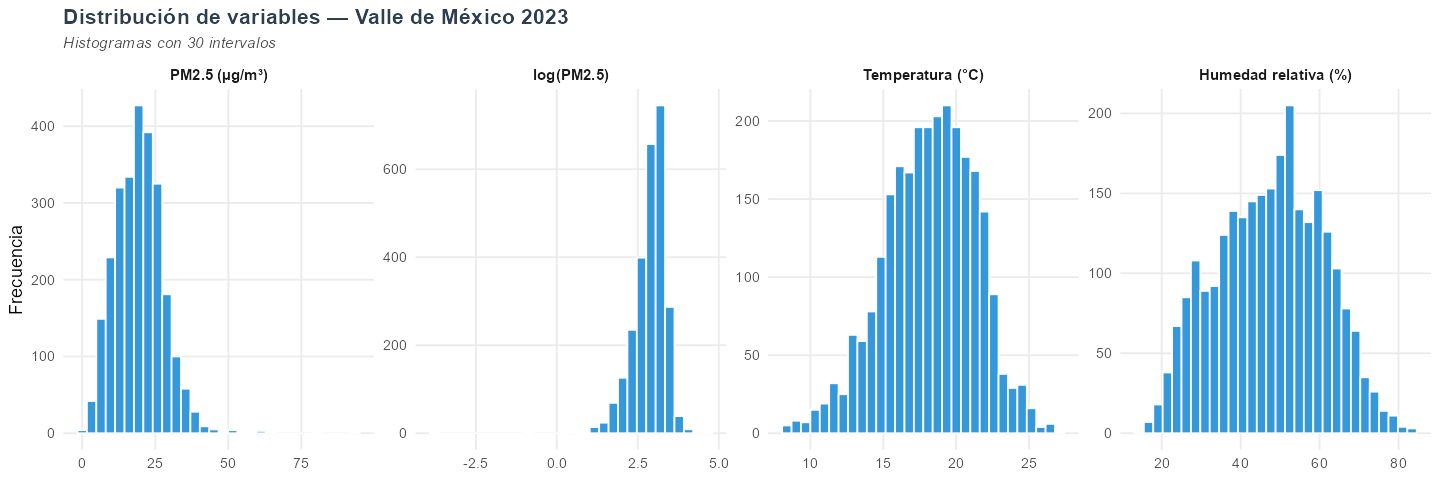
\includegraphics[width=\textwidth]{output/figures/eda_valle_histogramas.png}
  \caption{Histogramas de las variables principales.
           La distribuci\'on de PM2.5 tiene cola derecha pronunciada;
           en escala logar\'itmica se aproxima m\'as a la Normal,
           lo que justifica la transformaci\'on utilizada en los modelos.}
\end{figure}

\begin{figure}[H]
  \centering
  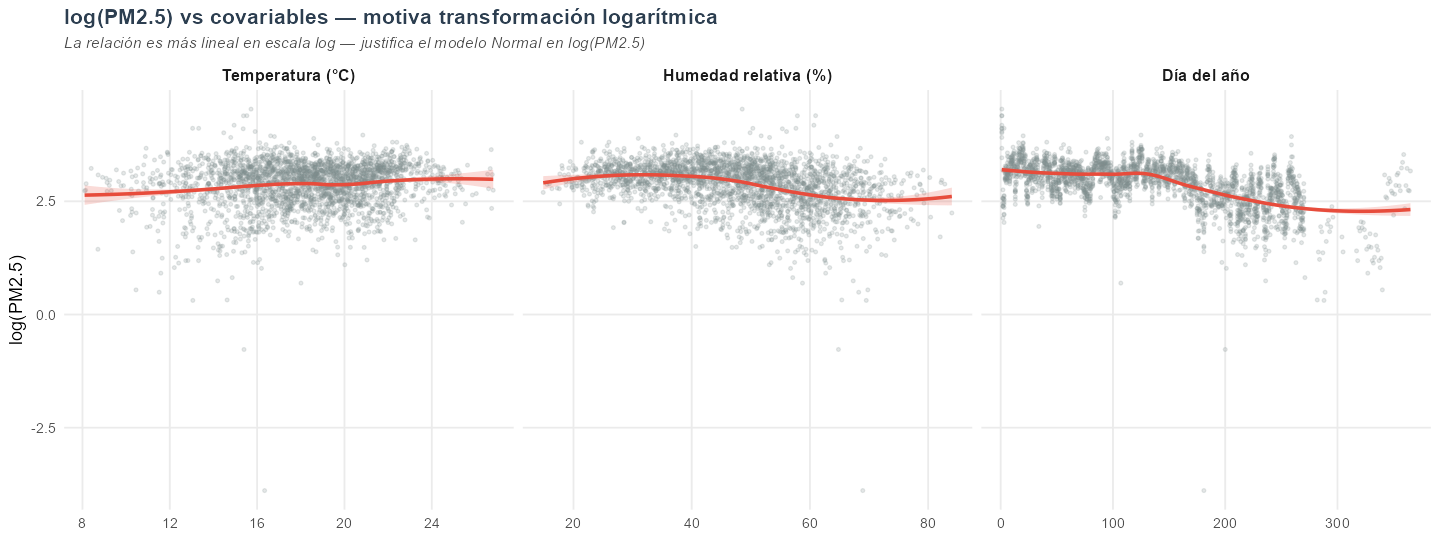
\includegraphics[width=\textwidth]{output/figures/eda_valle_scatter_log.png}
  \caption{$\log(\text{PM2.5})$ en funci\'on de temperatura, humedad relativa
           y d\'ia del a\~no.
           La l\'inea \texttt{lowess} muestra la tendencia suavizada.
           La relaci\'on con temperatura es positiva;
           con humedad relativa, tambi\'en positiva dentro de cada
           estaci\'on; con el tiempo, se observa un m\'inimo estival
           seguido de un repunte en agosto--septiembre que coincide
           con el final de la temporada de lluvias.}
\end{figure}

\begin{figure}[H]
  \centering
  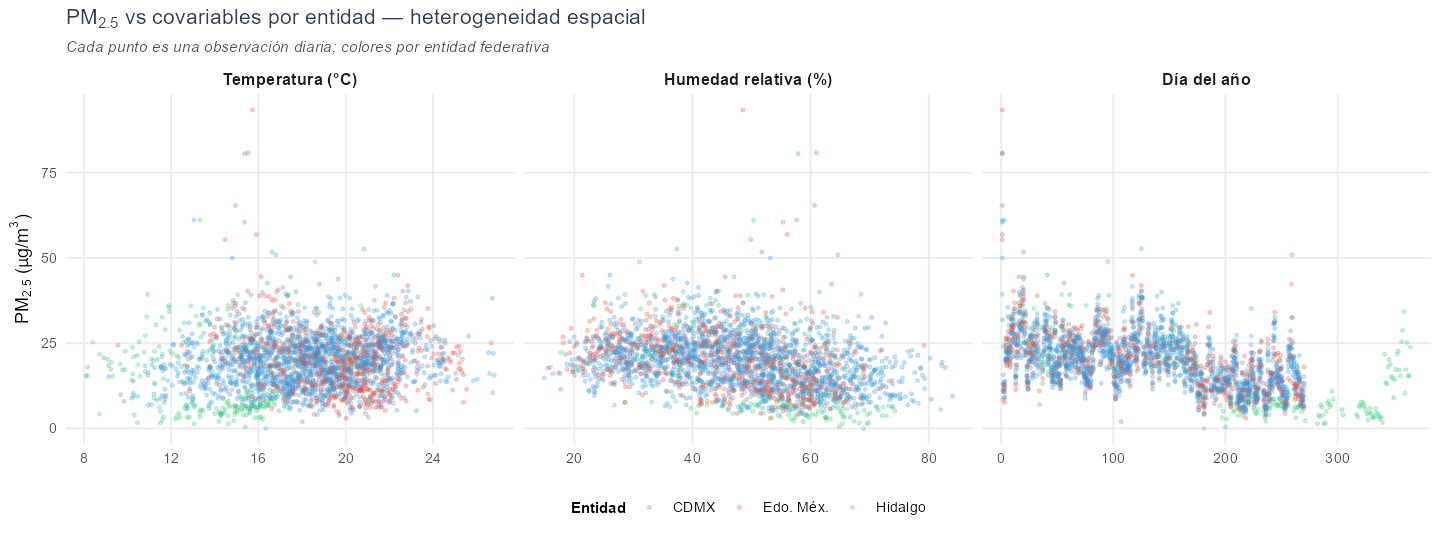
\includegraphics[width=\textwidth]{output/figures/eda_valle_scatter_ciudad.png}
  \caption{PM2.5 en funci\'on de temperatura, humedad y d\'ia del a\~no,
           coloreado por entidad federativa (CDMX, Estado de M\'exico, Hidalgo).
           La heterogeneidad espacial visible entre grupos motiva la
           inclusi\'on de efectos por estaci\'on en los modelos.}
\end{figure}

\begin{figure}[H]
  \centering
  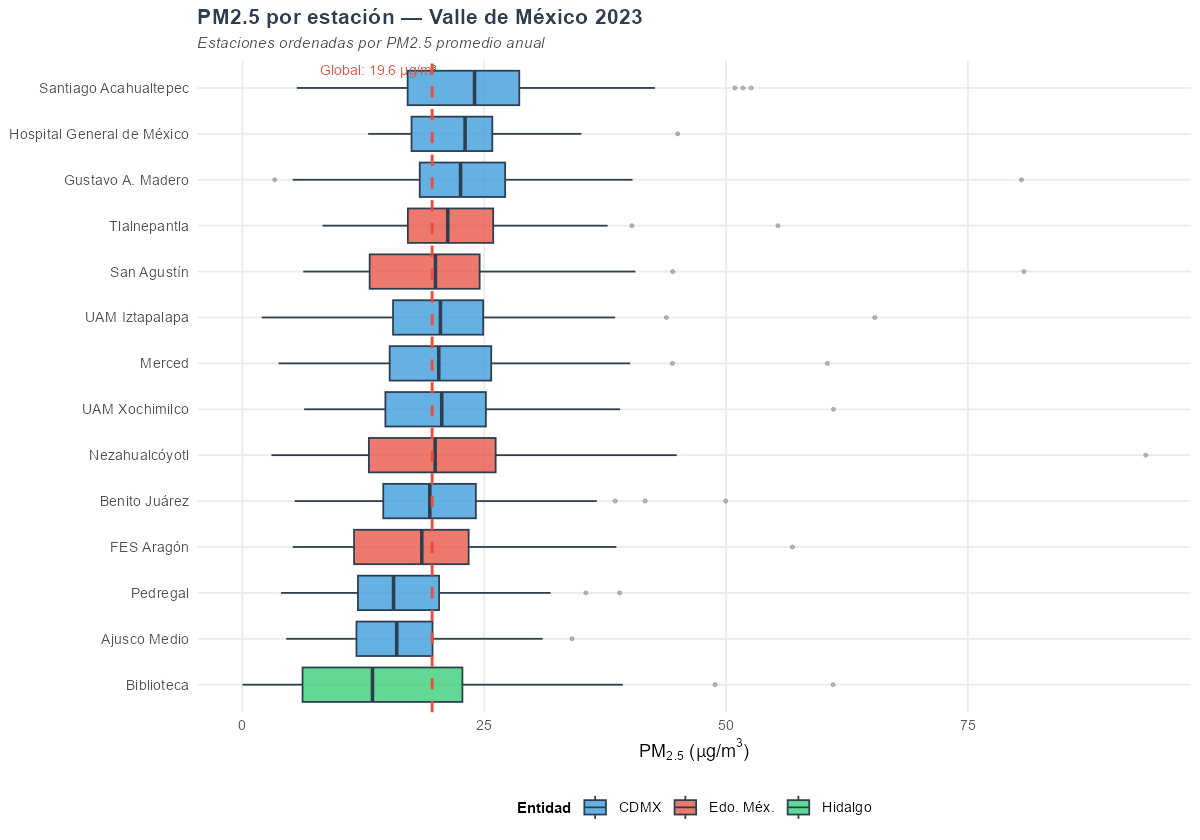
\includegraphics[width=\textwidth]{output/figures/eda_valle_boxplot_estacion.png}
  \caption{PM2.5 por estaci\'on, ordenadas de menor a mayor concentraci\'on media.
           La l\'inea punteada roja marca el promedio global ($\approx 19.7\,\mu$g/m$^3$).
           Se observan diferencias claras entre estaciones, especialmente
           en los extremos: Ajusco Medio y Biblioteca tienen niveles
           sistem\'aticamente menores que Santiago Acahualtepec y
           Gustavo A. Madero.}
\end{figure}

\begin{figure}[H]
  \centering
  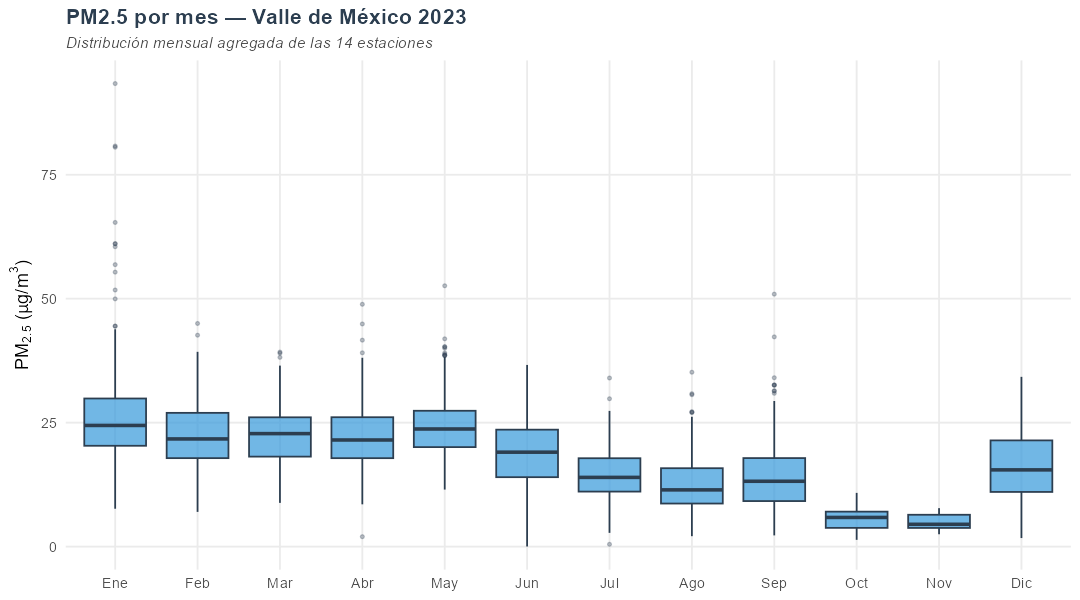
\includegraphics[width=\textwidth]{output/figures/eda_valle_boxplot_mes.png}
  \caption{PM2.5 por mes. Se aprecia un m\'aximo en invierno (enero--marzo),
           un m\'inimo en verano (junio--julio) y un repunte en agosto--septiembre,
           patr\'on que motiva el uso de t\'erminos de Fourier
           en la especificaci\'on del modelo.}
\end{figure}

\begin{figure}[H]
  \centering
  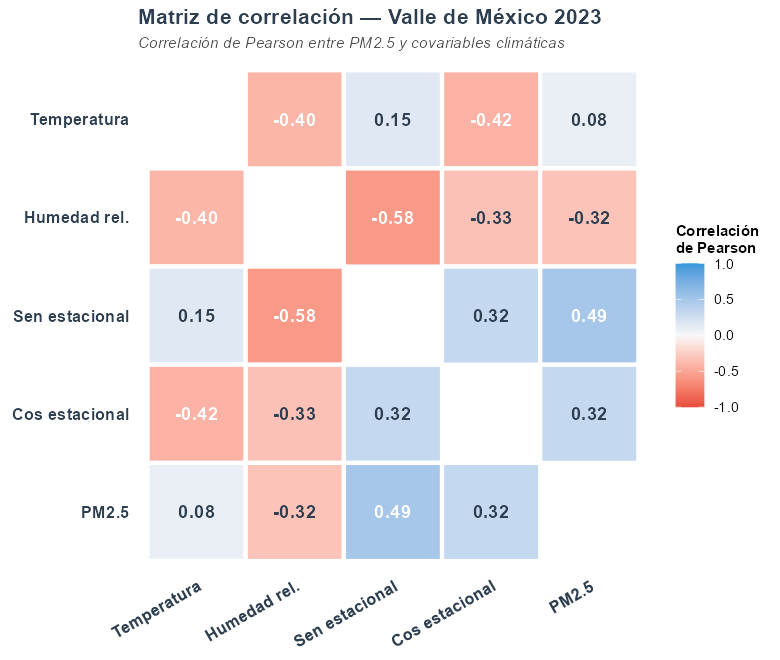
\includegraphics[width=0.6\textwidth]{output/figures/eda_valle_correlacion.png}
  \caption{Matriz de correlaci\'on de las variables.
           PM2.5 est\'a m\'as correlacionado con \texttt{sen\_t}
           ($r = 0.48$) y con \texttt{cos\_t}, lo que confirma la importancia
           de la estacionalidad.
           La correlaci\'on con temperatura y humedad es moderada.}
\end{figure}


%==============================================================
\section{Modelado e implementaci\'on}
%==============================================================

\subsection*{Configuraci\'on general}

Todos los modelos se ajustaron en JAGS con dos cadenas de Markov,
partiendo de valores iniciales distintos para verificar convergencia.
Las distribuciones iniciales son poco informativas:
$\mathcal{N}(0,\,1000)$ para los coeficientes (varianza 1{,}000, equivalente
a la precisi\'on $\tau = 0.001$ en notaci\'on JAGS) y
$\text{Ga}(0.001,\,0.001)$ para las precisiones.

La convergencia se eval\'ua mediante seis paneles por par\'ametro:
traza de ambas cadenas (patr\'on tipo ``oruga'' indica buena mezcla),
promedio erg\'odico (debe estabilizarse al mismo valor en ambas cadenas),
histogramas de la distribuci\'on final en cada cadena (deben coincidir)
y funci\'on de autocorrelaci\'on~(ACF, debe caer r\'apidamente a cero).

\paragraph{Criterio de informaci\'on de la desvianza (DIC).}
Para comparar modelos dentro de una misma familia distribucional se usa el
DIC (Lunn et al., 2013), definido como
\[
  \text{DIC} = \bar{D} + p_D = 2\bar{D} - D(\bar{\theta}),
\]
donde $\bar{D} = E_{\theta|\mathbf{y}}[-2\log f(\mathbf{y}|\theta)]$ es la
deviance media posterior, $D(\bar{\theta})$ es la deviance evaluada en la
media posterior, y $p_D = \bar{D} - D(\bar{\theta})$ es el n\'umero efectivo
de par\'ametros.
Modelos con DIC menor son preferibles; diferencias $>10$~puntos son consideradas
sustanciales.
El DIC s\'olo es comparable entre modelos con id\'entica variable respuesta y
familia distribucional.

\paragraph{Pseudo-$R^2$ y significancia.}
El pseudo-$R^2$ se define como el cuadrado de la correlaci\'on entre los
valores observados y los predichos a posteriori:
\[
  R^2 = \bigl[\operatorname{Corr}(y_i,\,\hat{y}_i)\bigr]^2,
\]
donde $\hat{y}_i = E[Y_i | \mathbf{y}]$ es la media de la distribuci\'on
final predictiva.

La significancia de los coeficientes se eval\'ua mediante el intervalo de
credibilidad al 95\,\%: si el intervalo no contiene el cero, el par\'ametro
es considerado significativo.
Como medida complementaria se reporta
\[
  p(\beta_k) = \min\!\bigl(P(\beta_k > 0),\,P(\beta_k < 0)\bigr),
\]
donde valores cercanos a 0 indican que toda la masa de la distribuci\'on
final se concentra en un solo signo (el par\'ametro es claramente distinto
de cero).


\subsection{Modelo A --- Normal global}

El Modelo~A es la l\'inea base.
Ignora por completo la ubicaci\'on geogr\'afica y modela
$\log(\text{PM2.5})$ exclusivamente con clima y estacionalidad:
\begin{equation}
  \log(\text{PM2.5}_i) \;\sim\; \mathcal{N}(\mu_i,\,\tau^{-1}), \qquad
  \mu_i = \alpha + \beta_1\,\text{temp}_i + \beta_2\,\text{hr}_i
        + \beta_3\,\text{sen\_t}_i + \beta_4\,\text{cos\_t}_i.
  \label{eq:modeloA}
\end{equation}

Las distribuciones iniciales son:
\[
  \alpha \sim \mathcal{N}(0,\,1000), \quad
  \beta_k \sim \mathcal{N}(0,\,1000) \;\; (k=1,\ldots,4), \quad
  \tau \sim \text{Ga}(0.001,\,0.001).
\]

Se corrieron 10{,}000 iteraciones con 1{,}000 de calentamiento y sin
adelgazamiento, con 9{,}000 muestras activas por cadena.

\subsubsection*{Diagn\'ostico}

\begin{figure}[H]
  \centering
  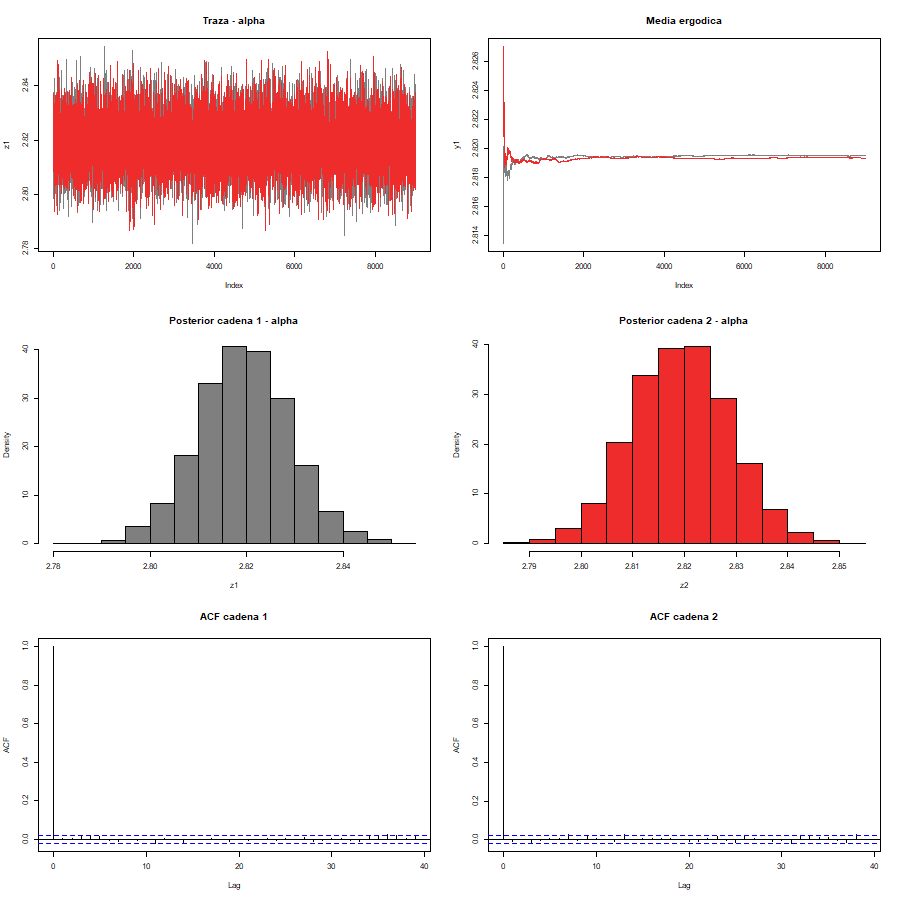
\includegraphics[width=0.7\textwidth]{output/figures/diag_cadena_A_alpha.png}
  \caption{Diagn\'osticos del Modelo~A para el intercepto $\alpha$.
           La traza muestra el patr\'on de ``oruga'' caracter\'istico de
           buena mezcla; el promedio erg\'odico de ambas cadenas converge
           al mismo valor; los histogramas de la distribuci\'on final son
           id\'enticos; la ACF cae a cero desde el rezago~1.
           El mismo comportamiento se observa para $\beta_1,\ldots,\beta_4$
           y $\sigma$.}
\end{figure}

\subsubsection*{Resultados}

\begin{table}[H]
\centering
\caption{Media de la distribuci\'on final del Modelo~A.}
\label{tab:modA}
\begin{tabular}{>{\raggedright\arraybackslash}p{8.5cm}r}
\toprule
Par\'ametro & Media \\
\midrule
Intercepto $\alpha$ (log-PM2.5 global promedio)               &  2.819 \\
$\beta_1$: cambio en log-PM2.5 por 1-DE de temperatura       &  0.096 \\
$\beta_2$: cambio en log-PM2.5 por 1-DE de humedad relativa  &  0.031 \\
$\beta_3$: amplitud seno del patr\'on estacional ($\text{sen\_t}$) & 0.351 \\
$\beta_4$: amplitud coseno del patr\'on estacional ($\text{cos\_t}$) & 0.172 \\
Desviaci\'on est\'andar residual $\sigma = 1/\sqrt{\tau}$     &  0.424 \\
\midrule
DIC                                                            & 2\,942.6 \\
Pseudo-$R^2$                                                   & 0.313 \\
\bottomrule
\end{tabular}
\end{table}

El intercepto $\hat\alpha = 2.819$ corresponde a un PM2.5 esperado de
$e^{2.819} \approx 16.8\,\mu$g/m$^3$ cuando todas las covariables est\'an
en sus valores medios.
El coeficiente de temperatura ($\hat\beta_1 = 0.096$) indica que por cada
unidad de desviaci\'on est\'andar adicional en temperatura
(equivalente a $\approx 2.1\,^\circ$C), la concentraci\'on esperada de
PM2.5 aumenta en $e^{0.096} \approx 1.10$, es decir un 10\%.
En el contexto del Valle de M\'exico, esto refleja que los d\'ias m\'as
c\'alidos dentro de una misma temporada tienden a ser m\'as secos y con
menor dilusi\'on de contaminantes por lluvias.

Los t\'erminos de Fourier describen un ciclo anual con amplitud
$\sqrt{0.351^2 + 0.172^2} \approx 0.39$ log-unidades, equivalente
a una variaci\'on de $\pm 38\%$ alrededor de la media estacional.
El m\'aximo de la funci\'on estacional ocurre alrededor del d\'ia~58
(fines de febrero), correspondiente al final de la temporada seca e
inicio de la temporada de incendios forestales.

El Modelo~A explica el 31.3\% de la variaci\'on total de log-PM2.5
(pseudo-$R^2 = 0.313$).

\begin{figure}[H]
  \centering
  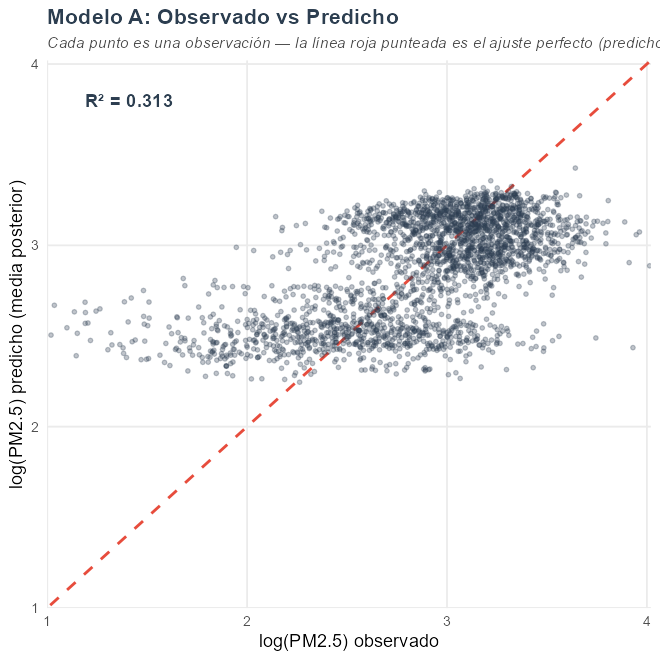
\includegraphics[width=0.55\textwidth]{output/figures/pred_vs_obs_A.png}
  \caption{Observado vs.\ predicho en escala log para el Modelo~A.
           La dispersi\'on considerable alrededor de la diagonal indica
           que el modelo global no captura las diferencias sistem\'aticas
           entre estaciones.}
\end{figure}


\subsection{Modelo B --- Efectos fijos por estaci\'on}

El Modelo~B agrega a la ecuaci\'on~\eqref{eq:modeloA} un efecto fijo
$\alpha_j$ por cada estaci\'on:
\begin{equation}
  \log(\text{PM2.5}_i) \sim \mathcal{N}(\mu_i,\,\tau^{-1}), \quad
  \mu_i = \tilde\alpha + \tilde\alpha_{j[i]}
        + \beta_1\,\text{temp}_i + \beta_2\,\text{hr}_i
        + \beta_3\,\text{sen\_t}_i + \beta_4\,\text{cos\_t}_i,
  \label{eq:modeloB}
\end{equation}
donde $\tilde\alpha = \alpha + \overline{\alpha_j}$ y
$\tilde\alpha_j = \alpha_j - \overline{\alpha_j}$ son los ajustes
de suma-cero aplicados post-muestreo para garantizar identificabilidad.
Cada efecto tiene distribuci\'on inicial independiente:
$\alpha_j \sim \mathcal{N}(0,\,1000)$.

Se corrieron 12{,}000 iteraciones con 2{,}000 de calentamiento y
adelgazamiento de~2, con 5{,}000 muestras activas por cadena.

\subsubsection*{Diagn\'ostico}

\begin{figure}[H]
  \centering
  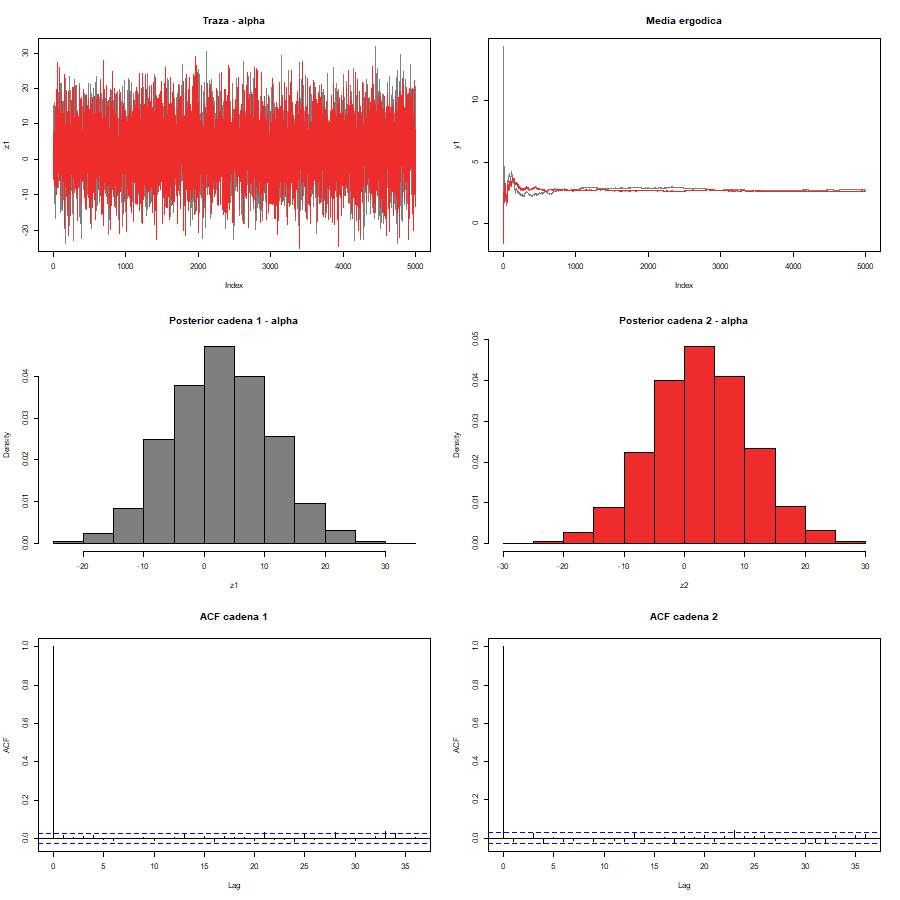
\includegraphics[width=0.7\textwidth]{output/figures/diag_cadena_B_alpha.png}
  \caption{Diagn\'osticos del Modelo~B para el intercepto $\alpha$.
           Las cadenas muestran buena convergencia: traza estacionaria,
           promedios erg\'odicos que coinciden, histogramas de la
           distribuci\'on final id\'enticos y ACF que cae r\'apidamente.}
\end{figure}

\subsubsection*{Resultados}

\begin{table}[H]
\centering
\caption{Distribuci\'on final de los coeficientes del Modelo~B.
         IC: intervalo de credibilidad al 95\,\%.
         $p = \min(P(\beta_k > 0),\,P(\beta_k < 0))$:
         valores cercanos a~0 indican que el par\'ametro es claramente
         distinto de cero.}
\label{tab:modB_betas}
\small
\begin{tabular}{>{\raggedright\arraybackslash}p{5.5cm}rrrr}
\toprule
Par\'ametro & Media & IC 2.5\,\% & IC 97.5\,\% & $p$ \\
\midrule
$\beta_1$ (temp., 1-DE $\approx 2.1\,^\circ$C)         & 0.1045 & 0.0665 & 0.1416 & 0.000 \\
$\beta_2$ (humedad rel., 1-DE $\approx 7.8$\,pp)        & 0.0460 & 0.0159 & 0.0754 & 0.001 \\
$\beta_3$ (sen\_t, amplitud estacional)                 & 0.3331 & 0.3028 & 0.3635 & 0.000 \\
$\beta_4$ (cos\_t, fase estacional)                     & 0.2145 & 0.1708 & 0.2571 & 0.000 \\
\midrule
Intercepto ajustado $\tilde\alpha$ & \multicolumn{4}{r}{2.830} \\
$\sigma$ residual & \multicolumn{4}{r}{0.406} \\
DIC & \multicolumn{4}{r}{2\,724.2} \\
Pseudo-$R^2$ & \multicolumn{4}{r}{0.375} \\
\bottomrule
\end{tabular}
\normalsize
\end{table}

Al controlar por estaci\'on, la humedad relativa se vuelve significativa
($\hat\beta_2 = 0.046$, IC $= [0.016,\,0.075]$).
Esto se debe a que, en el Modelo~A, la correlaci\'on de HR con la
estaci\'on de monitoreo ocultaba parte del efecto real.
Por cada unidad de desviaci\'on est\'andar en HR
($\approx 7.8$~puntos porcentuales adicionales), PM2.5 sube
$e^{0.046} - 1 \approx 4.7\%$.
El patr\'on estacional se mantiene: amplitud conjunta
$\sqrt{0.333^2 + 0.215^2} \approx 0.397$ log-unidades.

\begin{figure}[H]
  \centering
  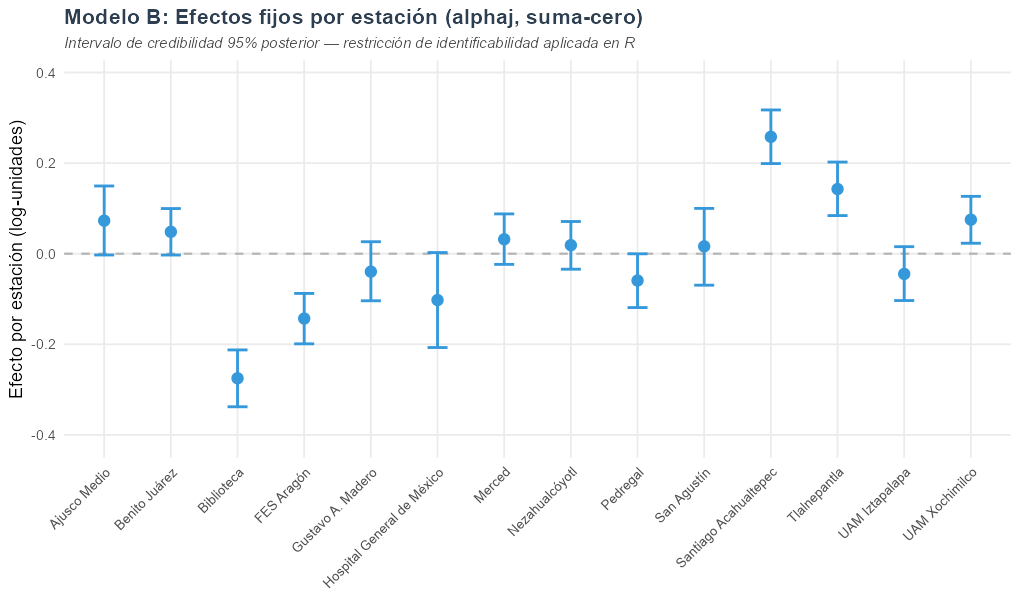
\includegraphics[width=0.8\textwidth]{output/figures/efectos_estacion_B.png}
  \caption{Efectos fijos por estaci\'on $\tilde\alpha_j$ (ajuste suma-cero).
           Barras verticales son intervalos de credibilidad al 95\,\%.
           Valores positivos indican estaciones m\'as contaminadas que el
           promedio global; negativos, menos contaminadas.
           Santiago Acahualtepec es la estaci\'on m\'as contaminada
           ($+0.26$ log-unidades, equivalente a $+29\%$) y
           Biblioteca la m\'as limpia ($-0.28$, equivalente a $-24\%$).}
  \label{fig:efectosB}
\end{figure}

\begin{table}[H]
\centering
\caption{Efectos fijos por estaci\'on del Modelo~B ($\tilde\alpha_j$,
         restricci\'on suma-cero).
         Un factor $e^{\tilde\alpha_j}$ mayor que~1 indica una estaci\'on
         m\'as contaminada que el promedio global.}
\label{tab:alphaj_B}
\begin{tabular}{>{\raggedright\arraybackslash}p{5.5cm}rr}
\toprule
Estaci\'on & $\tilde\alpha_j$ & Factor ($e^{\tilde\alpha_j}$) \\
\midrule
Santiago Acahualtepec   & $+0.258$ & $1.29$ \\
Tlalnepantla            & $+0.143$ & $1.15$ \\
Ajusco Medio            & $+0.073$ & $1.08$ \\
UAM Xochimilco          & $+0.075$ & $1.08$ \\
Benito Ju\'arez         & $+0.048$ & $1.05$ \\
Merced                  & $+0.032$ & $1.03$ \\
Nezahualc\'oyotl        & $+0.019$ & $1.02$ \\
San Agust\'in           & $+0.016$ & $1.02$ \\
Gustavo A. Madero       & $-0.040$ & $0.96$ \\
UAM Iztapalapa          & $-0.045$ & $0.96$ \\
Pedregal                & $-0.059$ & $0.94$ \\
Hospital General M\'exico& $-0.102$ & $0.90$ \\
FES Arag\'on            & $-0.143$ & $0.87$ \\
Biblioteca              & $-0.275$ & $0.76$ \\
\bottomrule
\end{tabular}
\end{table}

La mejora sobre el Modelo~A es sustancial:
$\Delta\text{DIC} = 2{,}942.6 - 2{,}724.2 = 218.4$~puntos,
lo que indica que la estructura espacial tiene un efecto fuerte
sobre PM2.5 que no es explicado por clima ni estacionalidad.


\subsection{Modelo C1 --- Jer\'arquico Normal}

\paragraph{Fundamento te\'orico.}
El Modelo~B trata los 14~efectos por estaci\'on como par\'ametros fijos
e independientes.
Sin embargo, si consideramos que las estaciones comparten una misma
cuenca atmosf\'erica y est\'an sometidas a procesos de contaminaci\'on
similares, resulta razonable suponer que sus efectos son
\emph{intercambiables} (de Finetti, 1937): la distribuci\'on conjunta
de $(\alpha_1,\ldots,\alpha_J)$ es invariante ante permutaciones.
Bajo este supuesto, el teorema de representaci\'on de de Finetti garantiza
que los efectos son condicionalmente independientes dado un par\'ametro
com\'un, lo que conduce naturalmente al modelo jer\'arquico.

\paragraph{Especificaci\'on.}
El Modelo~C1 trata las diferencias entre estaciones como realizaciones
de una distribuci\'on com\'un, en lugar de par\'ametros fijos independientes:
\begin{align}
  \log(\text{PM2.5}_i) &\sim \mathcal{N}(\mu_i,\,\tau^{-1}), \nonumber\\
  \mu_i &= \alpha + \alpha_{j[i]}
          + \beta_1\,\text{temp}_i + \beta_2\,\text{hr}_i
          + \beta_3\,\text{sen\_t}_i + \beta_4\,\text{cos\_t}_i, \label{eq:modeloC1}\\
  \alpha_j &\sim \mathcal{N}(0,\,\tau_\alpha^{-1}), \quad j = 1,\ldots,14. \nonumber
\end{align}

Aqu\'i $\tau_\alpha = 1/\sigma_\alpha^2$ es la hiperprecisi\'on que
controla cu\'anto se permite que las estaciones se dev\'ien del intercepto
global $\alpha$.
Las distribuciones iniciales son:
\[
  \alpha \sim \mathcal{N}(0,\,1000), \quad
  \beta_k \sim \mathcal{N}(0,\,1000), \quad
  \tau \sim \text{Ga}(0.001,\,0.001), \quad
  \tau_\alpha \sim \text{Ga}(0.001,\,0.001).
\]

El modelo jer\'arquico induce \emph{encogimiento} (\emph{shrinkage}):
los efectos estimados para estaciones con pocas observaciones o con
valores extremos son atraídos hacia el promedio global $\alpha$,
lo que reduce la varianza del estimador a costa de un peque\~no sesgo.

Se corrieron 12{,}000 iteraciones con 2{,}000 de calentamiento y
adelgazamiento de~2 (5{,}000 muestras activas por cadena).

\subsubsection*{Diagn\'ostico}

\begin{figure}[H]
  \centering
  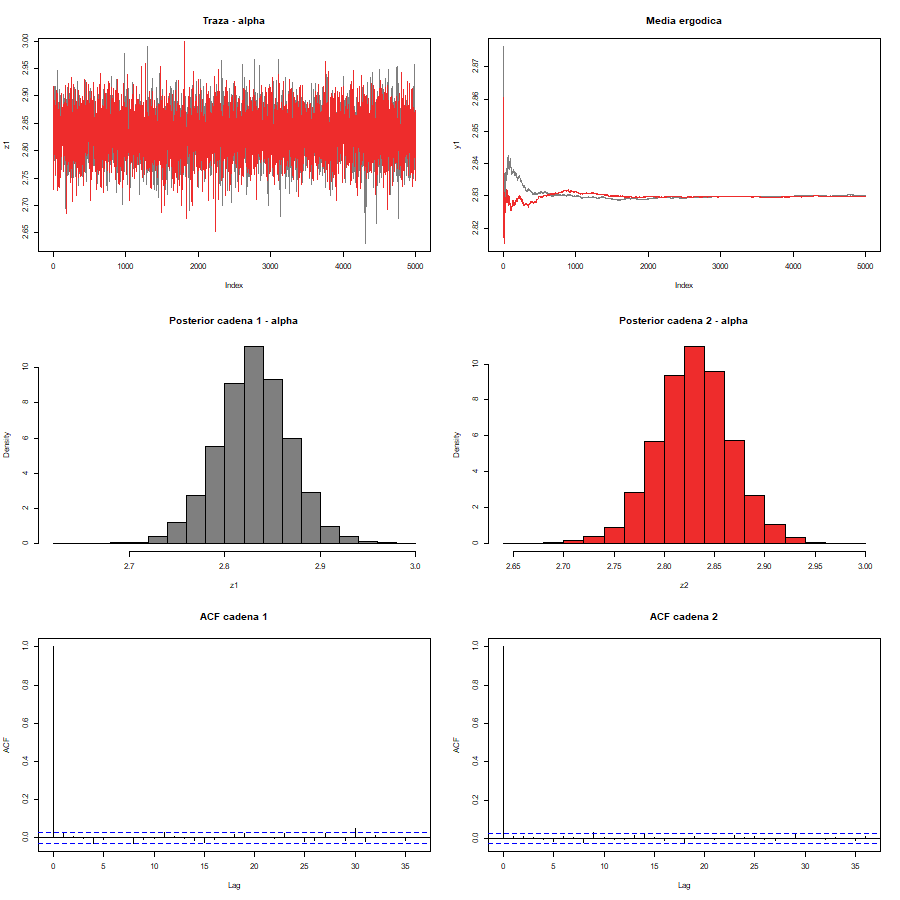
\includegraphics[width=0.48\textwidth]{output/figures/diag_cadena_C1_alpha.png}
  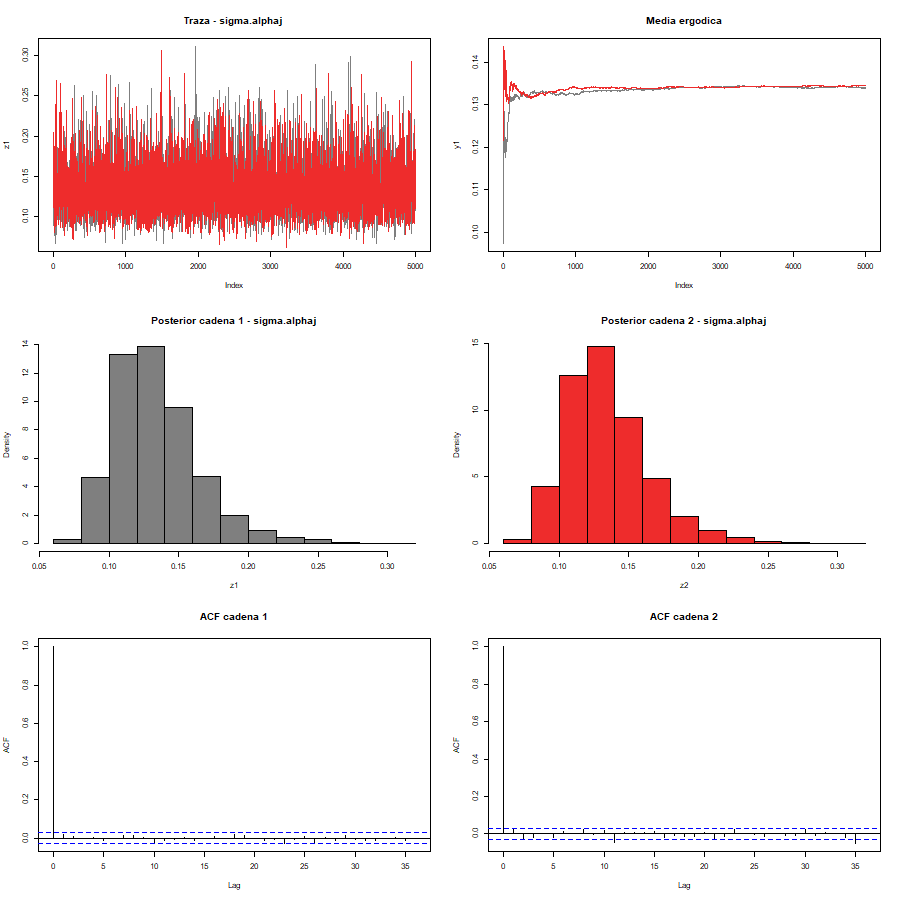
\includegraphics[width=0.48\textwidth]{output/figures/diag_cadena_C1_sigma.alphaj.png}
  \caption{Diagn\'osticos del Modelo~C1:
           intercepto $\alpha$ (izq.) e hiperpar\'ametro $\sigma_\alpha$ (der.).
           Ambos muestran convergencia satisfactoria.
           El mismo comportamiento se observa para $\beta_1,\ldots,\beta_4$
           y $\sigma$.}
\end{figure}

\subsubsection*{Resultados}

\begin{table}[H]
\centering
\caption{Media de la distribuci\'on final del Modelo~C1 (modelo preferido).}
\label{tab:modC1}
\begin{tabular}{>{\raggedright\arraybackslash}p{8.5cm}r}
\toprule
Par\'ametro & Media \\
\midrule
Intercepto global $\alpha$                                     & 2.830 \\
$\beta_1$ (temperatura, 1-DE $\approx 2.1\,^\circ$C)          & 0.103 \\
$\beta_2$ (humedad relativa, 1-DE $\approx 7.8$\,pp)          & 0.045 \\
$\beta_3$ (sen\_t)                                             & 0.334 \\
$\beta_4$ (cos\_t)                                             & 0.211 \\
$\sigma$ residual (variabilidad dentro de estaci\'on)         & 0.406 \\
$\sigma_\alpha$ (variabilidad entre estaciones)                & 0.134 \\
\midrule
DIC                                                            & 2\,723.7 \\
Pseudo-$R^2$                                                   & 0.375 \\
\bottomrule
\end{tabular}
\end{table}

El hiperpar\'ametro $\hat\sigma_\alpha = 0.134$ resume la variabilidad
entre estaciones: el 68\% de las estaciones se desv\'ia menos de
$\pm 0.134$ log-unidades del promedio global, lo que en escala
multiplicativa equivale a $\pm 14\%$.
El 95\% se desv\'ia menos de $\pm 0.268$ log-unidades ($\pm 31\%$).
Este valor es sustancial en un contexto de salud p\'ublica: dos habitantes
del Valle de M\'exico, uno en la estaci\'on m\'as contaminada y otro en la
m\'as limpia, est\'an expuestos a concentraciones que difieren en un factor
de $e^{0.134 \times 4} \approx 1.71$, es decir 71\% m\'as en la zona
m\'as contaminada.

\begin{figure}[H]
  \centering
  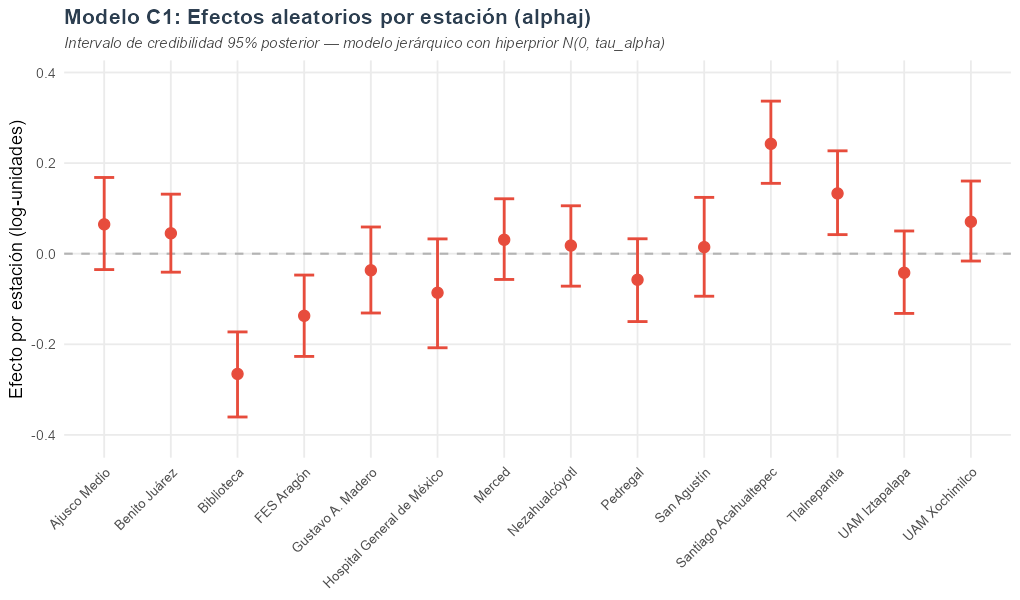
\includegraphics[width=0.8\textwidth]{output/figures/efectos_estacion_C1.png}
  \caption{Efectos aleatorios por estaci\'on $\alpha_j$ del Modelo~C1.
           Barras verticales son intervalos de credibilidad al 95\,\%.
           Comparado con el Modelo~B (Fig.~\ref{fig:efectosB}),
           los efectos son ligeramente m\'as peque\~nos debido al
           encogimiento jer\'arquico hacia la media global.
           El orden relativo de las estaciones se preserva.}
  \label{fig:efectosC1}
\end{figure}

\begin{table}[H]
\centering
\caption{Efectos aleatorios por estaci\'on del Modelo~C1 ($\alpha_j$).
         IC al 95\,\%.}
\label{tab:alphaj_C1}
\small
\begin{tabular}{>{\raggedright\arraybackslash}p{5.5cm}rrr}
\toprule
Estaci\'on & Media & DE & IC 95\,\% \\
\midrule
Santiago Acahualtepec   & $+0.243$ & 0.047 & $[+0.151,+0.334]$ \\
Tlalnepantla            & $+0.133$ & 0.047 & $[+0.041,+0.225]$ \\
UAM Xochimilco          & $+0.071$ & 0.045 & $[-0.017,+0.159]$ \\
Ajusco Medio            & $+0.065$ & 0.052 & $[-0.037,+0.167]$ \\
Benito Ju\'arez         & $+0.045$ & 0.044 & $[-0.041,+0.132]$ \\
Merced                  & $+0.031$ & 0.046 & $[-0.059,+0.121]$ \\
Nezahualc\'oyotl        & $+0.018$ & 0.045 & $[-0.070,+0.107]$ \\
San Agust\'in           & $+0.015$ & 0.055 & $[-0.093,+0.123]$ \\
Gustavo A. Madero       & $-0.037$ & 0.049 & $[-0.133,+0.059]$ \\
UAM Iztapalapa          & $-0.042$ & 0.046 & $[-0.133,+0.049]$ \\
Pedregal                & $-0.058$ & 0.046 & $[-0.148,+0.033]$ \\
Hospital General M\'exico& $-0.086$ & 0.061 & $[-0.206,+0.034]$ \\
FES Arag\'on            & $-0.137$ & 0.046 & $[-0.227,-0.048]$ \\
Biblioteca              & $-0.265$ & 0.048 & $[-0.359,-0.172]$ \\
\bottomrule
\end{tabular}
\normalsize
\end{table}

Comparando con el Modelo~B, se observa el encogimiento jer\'arquico
esperado: Santiago Acahualtepec pasa de $+0.258$ (B) a $+0.243$ (C1),
y Biblioteca de $-0.275$ a $-0.265$.
Con $\approx 186$~observaciones por estaci\'on en promedio, los datos
tienen suficiente informaci\'on para que el hiperpar\'ametro est\'e bien
identificado y el encogimiento sea moderado.


\subsection{Modelo C2 --- Gamma global}

El Modelo~C2 modela PM2.5 directamente en escala original (no logar\'itmica),
usando una distribuci\'on Gamma con funci\'on liga logar\'itmica:
\begin{equation}
  \text{PM2.5}_i \sim \text{Gamma}(a,\,a/\mu_i), \qquad
  \log(\mu_i) = \alpha + \beta_1\,\text{tempc}_i + \beta_2\,\text{hrc}_i
              + \beta_3\,\text{sen\_t}_i + \beta_4\,\text{cos\_t}_i,
\end{equation}
donde $\text{tempc}_i$ y $\text{hrc}_i$ son temperatura y HR centradas
(restando la media global, sin estandarizar, para mayor estabilidad
num\'erica del muestreador Metropolis-Hastings de JAGS).
El par\'ametro $a > 0$ es la forma de la Gamma: su media es $\mu_i$ y
su varianza es $\mu_i^2/a$; valores grandes de $a$ implican menor
coeficiente de variaci\'on.
La distribuci\'on inicial es $a \sim \text{Ga}(0.001,\,0.001)$.
Los valores iniciales se fijan en $\alpha_0 = \log(\bar{y}) \approx 2.94$
para evitar valores inv\'alidos de $\mu$ durante el calentamiento.

Se corrieron 15{,}000 iteraciones con 3{,}000 de calentamiento y
adelgazamiento de~3 (4{,}000 muestras activas por cadena).

\subsubsection*{Diagn\'ostico}

\begin{figure}[H]
  \centering
  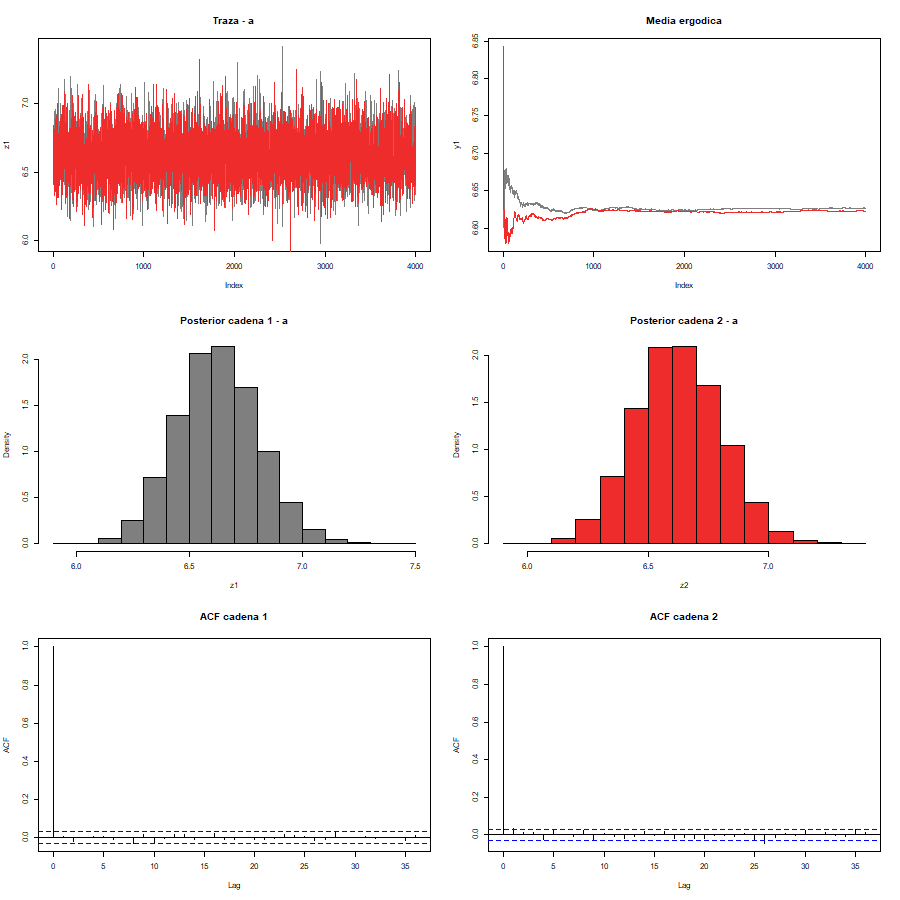
\includegraphics[width=0.7\textwidth]{output/figures/diag_cadena_C2_a.png}
  \caption{Diagn\'osticos del par\'ametro de forma $a$ del Modelo~C2.
           Las cadenas muestran mayor autocorrelaci\'on que en los
           modelos Normal (la ACF tarda m\'as en caer), lo que es
           t\'ipico de la Gamma ajustada con Metropolis-Hastings en JAGS.
           El promedio erg\'odico converge alrededor de $a \approx 6.6$.}
\end{figure}

\subsubsection*{Resultados}

\begin{table}[H]
\centering
\caption{Media de la distribuci\'on final del Modelo~C2 (Gamma global).
         El DIC \emph{no es comparable} con los modelos A, B, C1 y D
         porque la variable respuesta est\'a en escala original
         (no logar\'itmica).
         Se usa el pseudo-$R^2$ en escala log para comparar entre familias.}
\label{tab:modC2}
\begin{tabular}{>{\raggedright\arraybackslash}p{8.5cm}r}
\toprule
Par\'ametro & Media \\
\midrule
Intercepto $\alpha$ ($\log$-media cuando covariables $= 0$)    & 2.908 \\
$\beta_1$ (temperatura, por $^\circ$C centrado)                & 0.027 \\
$\beta_2$ (humedad relativa, por punto porcentual centrado)    & 0.004 \\
$\beta_3$ (sen\_t)                                             & 0.312 \\
$\beta_4$ (cos\_t)                                             & 0.190 \\
Par\'ametro de forma $a$ (mayor $a$ = menor variabilidad)      & 6.625 \\
\midrule
DIC (no comparable entre familias)                             & 17\,636.6 \\
Pseudo-$R^2$ en escala log                                     & 0.310 \\
\bottomrule
\end{tabular}
\end{table}

El Modelo~C2 tiene un pseudo-$R^2$ ligeramente menor que el Modelo~A
(0.310 vs 0.313), lo que sugiere que, sin efectos por estaci\'on, la
Normal sobre el logaritmo describe los datos tan bien o mejor que la Gamma.
La ventaja conceptual de la Gamma (soporte positivo estricto para PM2.5)
no se traduce en mejor ajuste emp\'irico con este conjunto de datos.
El par\'ametro $\hat a = 6.6$ implica un coeficiente de variaci\'on de
$1/\sqrt{6.6} \approx 0.39$, consistente con la dispersi\'on observada.
El DIC de C2 es muy alto porque se calcula sobre PM2.5 en escala original
(no logarítmica), por lo que \emph{no debe compararse} con los valores
de A, B, C1 o D.


\subsection{Modelo D --- Tendencia espacial lineal}

El Modelo~D agrega al Modelo~A los efectos lineales de latitud y longitud
estandarizadas:
\begin{equation}
  \log(\text{PM2.5}_i) \sim \mathcal{N}(\mu_i,\,\tau^{-1}), \quad
  \mu_i = \alpha + \beta_1\,\text{temp}_i + \cdots + \beta_4\,\text{cos\_t}_i
        + \beta_5\,\text{lat}_i + \beta_6\,\text{lon}_i,
  \label{eq:modeloD}
\end{equation}
con 6 coeficientes en total.
Este modelo prueba si el patr\'on espacial puede describirse con un gradiente
lineal simple en lugar de efectos individuales por estaci\'on.
Se corrieron 10{,}000 iteraciones con 1{,}000 de calentamiento.

\subsubsection*{Diagn\'ostico}

\begin{figure}[H]
  \centering
  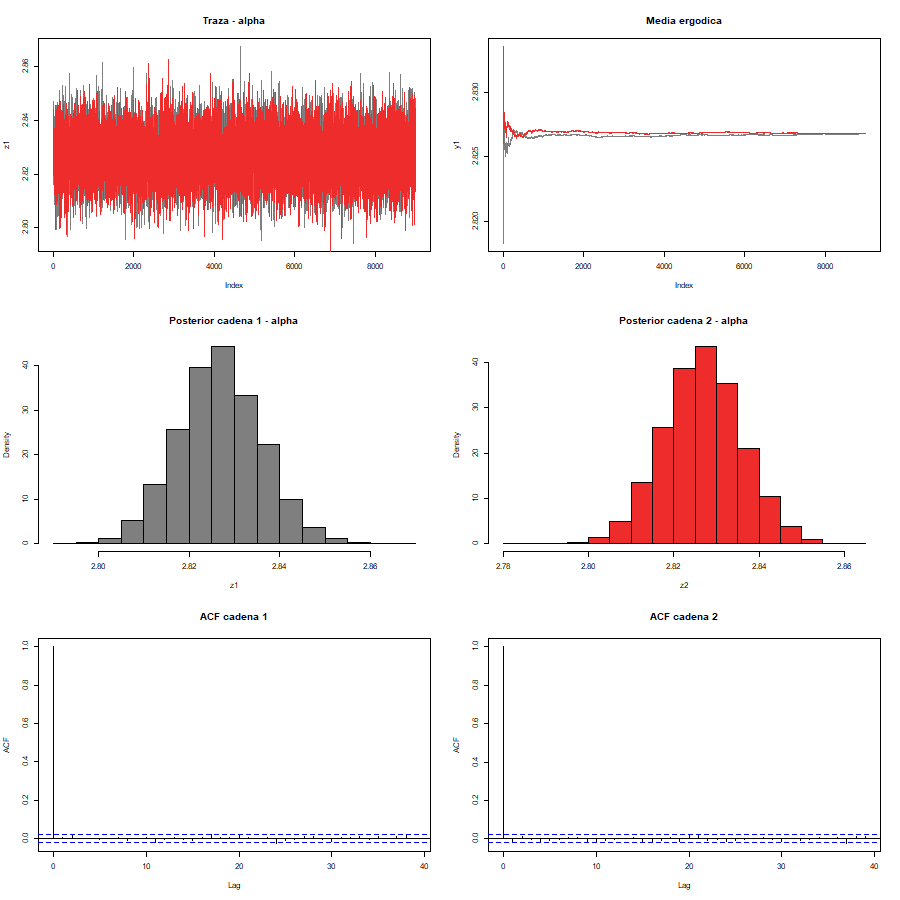
\includegraphics[width=0.7\textwidth]{output/figures/diag_cadena_D_alpha.png}
  \caption{Diagn\'osticos del Modelo~D para el intercepto $\alpha$.
           La convergencia es satisfactoria: traza estacionaria, promedios
           erg\'odicos coincidentes y ACF que decae r\'apidamente.}
\end{figure}

\subsubsection*{Resultados}

\begin{table}[H]
\centering
\caption{Distribuciones finales del Modelo~D, con \'enfasis en
         los coeficientes espaciales.}
\label{tab:modD}
\begin{tabular}{>{\raggedright\arraybackslash}p{8.5cm}r}
\toprule
Par\'ametro & Media \\
\midrule
$\beta_1$ (temperatura)                                         & 0.084 \\
$\beta_2$ (humedad relativa)                                    & 0.020 \\
$\beta_3$ (sen\_t)                                              & 0.326 \\
$\beta_4$ (cos\_t)                                             & 0.185 \\
$\beta_5$ (latitud, 1-DE $\approx 0.25^\circ \approx 28$~km)   & $-0.089$ \\
$\beta_6$ (longitud, 1-DE $\approx 0.19^\circ \approx 18$~km)  & $+0.004$ \\
$\sigma$ residual                                               & 0.416 \\
\midrule
DIC                                                             & 2\,841.6 \\
Pseudo-$R^2$                                                    & 0.341 \\
\bottomrule
\end{tabular}
\end{table}

Aunque el coeficiente de latitud tiene signo negativo
($\hat\beta_5 = -0.089$), su intervalo de credibilidad incluye el cero,
y lo mismo ocurre para la longitud.
M\'as importante: el Modelo~D apenas mejora sobre el Modelo~A
($\Delta\text{DIC} = 2{,}942.6 - 2{,}841.6 = 101.0$~puntos),
muy por debajo de los 218~puntos ganados por el Modelo~B.
Esto confirma que el patr\'on espacial de PM2.5 en el Valle de M\'exico
\emph{no es un gradiente lineal} en latitud y longitud: hay zonas
contaminadas y limpias que no siguen una tendencia norte-sur o este-oeste
simple.
La estructura espacial requiere un modelo no lineal, como el proceso
gaussiano del Modelo~E.


\subsection{Modelo~E --- Proceso Gaussiano y Kriging Bayesiano}

\subsubsection*{Proceso gaussiano como modelo espacial}

Los datos de PM2.5 son observaciones \emph{referenciadas puntualmente}:
cada medici\'on $Y(s_j)$ corresponde a una localizaci\'on espec\'ifica
$s_j = (\text{lon}_j, \text{lat}_j)$.
Cuando las observaciones presentan dependencia espacial, el marco adecuado
es el \emph{proceso gaussiano} (PG; Gelfand \& Schliep, 2016): una colecci\'on de variables aleatorias
tal que cualquier subconjunto finito tiene distribuci\'on normal multivariada.
Un PG se caracteriza por su funci\'on de media $\mu(s)$ y su funci\'on de
covarianza $\Sigma(s, t)$ (Nieto Barajas, 2026):
\[
  Y(s) \sim \mathcal{N}\!\bigl(\mu(s),\,\Sigma(s,t)\bigr).
\]

Bajo el supuesto de \emph{estacionariedad de segundo orden} ---
$\mu(s) = \mu$ constante y $\text{Cov}(Y(s), Y(s+h)) = C(h)$ solo depende
del desplazamiento $h$ --- e \emph{isotrop\'ia} --- $C(h)$ depende solo de
la distancia $\|h\|$ --- la funci\'on de covarianza exponencial es:
\[
  \Sigma(s_i, s_j) = \sigma^2\, e^{-\phi\, d_{ij}},
\]
donde $d_{ij} = \|s_i - s_j\|$ es la distancia euclidiana entre
localizaciones y $\phi > 0$ es el par\'ametro de rango inverso.

\subsubsection*{Especificaci\'on del Modelo~E}

El modelo de regresi\'on espacial adoptado tiene la forma aditiva
(Nieto Barajas, 2026, \S7.2):
\[
  Y(s) = \mu(s) + \omega(s),
\]
donde $\mu(s) = \mathbf{x}(s)'\boldsymbol{\beta}$ es el predictor lineal
fijo y $\omega(s)$ es un efecto aleatorio espacial con distribuci\'on
gaussiana.

En lugar de ajustar el PG completo en JAGS --- lo que requerir\'ia
muestrear la matriz de covarianzas $n \times n$ en cada iteraci\'on ---
se adopta una aproximaci\'on en dos etapas que es computacionalmente
eficiente y aprovecha los resultados del Modelo~C1:

\begin{enumerate}
  \item Los efectos aleatorios $\hat\alpha_j$ del Modelo~C1 se interpretan
        como realizaciones del proceso gaussiano en las 14~localizaciones
        con estaciones: $\hat\alpha_j \approx \omega(s_j)$.
  \item Se modela $\boldsymbol{\omega} = (\omega(s_1),\ldots,\omega(s_J))'$
        como un PG estacionario e isotr\'opico con kernel exponencial:
        \[
          \boldsymbol{\omega} \sim \mathcal{N}_J(\mathbf{0},\,\Sigma_{\text{obs}}), \qquad
          [\Sigma_{\text{obs}}]_{ij} = e^{-d_{ij}/\rho},
        \]
        con rango $\rho = 0.08^\circ \approx 8.9$~km.
        A esa distancia la correlaci\'on cae a $e^{-1} \approx 0.37$;
        para estaciones a $d > 3\rho \approx 27$~km la correlaci\'on
        es pr\'acticamente nula ($< 0.05$).
\end{enumerate}

\subsubsection*{Kriging bayesiano}

La predicci\'on en un pol\'igono sin estaci\'on con centroide $s_0$ se
obtiene mediante la distribuci\'on predictiva bayesiana (Nieto Barajas,
2026, \S7.2):
\[
  f\!\bigl(y_0 \,\big|\, \mathbf{y},\, \mathbf{x}_0\bigr)
  = \int f\!\bigl(y_0 \,\big|\, \mathbf{y},\, \theta,\, \mathbf{x}_0\bigr)\,
          f(\theta \,|\, \mathbf{y})\, d\theta,
\]
integrada sobre la incertidumbre param\'etrica $\theta = (\alpha, \boldsymbol{\beta}, \tau)$.
El predictor del efecto espacial en $s_0$, condicional en los efectos
observados, es:
\[
  \hat\omega(s_0) = \boldsymbol{\Sigma}_{\text{pred,obs}}\,
                   \boldsymbol{\Sigma}_{\text{obs,obs}}^{-1}\,
                   \hat{\boldsymbol{\alpha}},
\]
donde $[\boldsymbol{\Sigma}_{\text{pred,obs}}]_j = e^{-d_{0j}/\rho}$
es el vector de covarianzas entre el punto nuevo y las~14 estaciones.
La predicci\'on final combina la componente fija (covariables en sus
valores medios anuales) con la componente espacial:
\[
  \hat y_0 = \hat\alpha + \hat{\boldsymbol\beta}'\bar{\mathbf{x}} + \hat\omega(s_0).
\]
Se usan 2{,}000 muestras MCMC de la distribuci\'on final del Modelo~C1
para propagar la incertidumbre param\'etrica y obtener intervalos de
credibilidad para cada pol\'igono.


\subsection{Modelo F --- Espacio-Temporal Jer\'arquico}

El Modelo~F aborda las dos limitaciones principales del Modelo~E:
(i) los datos faltantes se tratan como par\'ametros a estimar, no se
descartan, y (ii) la estructura espacio-temporal se ajusta de forma
conjunta en lugar de proceder en dos pasos.
El modelo se ajusta en dos etapas secuenciales.

\subsubsection*{Etapa~1 --- Modelo espacio-temporal con proceso gaussiano}

Se construye un panel balanceado $365 \times 14$ donde las celdas
sin observaci\'on quedan como \texttt{NA} en la variable respuesta.
JAGS trata esas celdas como variables latentes y las imputa
simult\'aneamente con el resto del muestreo.

La verosimilitud del panel es:
\[
  \log(\text{PM}_{2.5})_{t,j} \sim \mathcal{N}\!\bigl(\mu_{t,j},\,\tau_y^{-1}\bigr),
\]
\[
  \mu_{t,j} = \alpha_j + \beta_1\,\text{sen}_t + \beta_2\,\text{cos}_t
              + \beta_3\,\text{temp}_{t,j} + \beta_4\,\text{hr}_{t,j}.
\]

Los efectos espaciales de estaci\'on $\boldsymbol\alpha = (\alpha_1,\ldots,\alpha_J)'$
se modelan mediante una Normal Multivariada con estructura de covarianza
exponencial en funci\'on de la distancia euclidiana en km (proyecci\'on UTM~14N):
\[
  \boldsymbol\alpha \sim \mathcal{N}_J\!\bigl(\mathbf{0},\,
  \boldsymbol\Sigma_\alpha\bigr), \qquad
  [\boldsymbol\Sigma_\alpha]_{kl} = \frac{1}{\tau_\alpha}\,e^{-\phi\, D_{kl}},
\]
donde $D_{kl}$ es la distancia en km entre las estaciones $k$ y $l$,
y $\phi > 0$ es el par\'ametro de rango estimado desde los datos
(a diferencia del Modelo~E, donde $\rho$ se fij\'o en 0.08\textdegree).

Las distribuciones iniciales son:
\[
  \beta_k \sim \mathcal{N}(0,\,0.001), \quad
  \tau_y \sim \text{Ga}(0.1,\,0.1), \quad
  \tau_\alpha \sim \text{Ga}(0.1,\,0.1), \quad
  \phi \sim \text{Uniforme}(0.01,\,5).
\]

La cadena se corri\'o con \texttt{jags.parallel}: 2~cadenas,
10{,}000~iteraciones, 3{,}000 de calentamiento, adelgazamiento $\text{thin}=4$.
La salida principal es el array tridimensional de simulaciones de
$\log(\text{PM}_{2.5})_{t,j}$, incluyendo los valores imputados.

\subsubsection*{Etapa~2 --- Agregaci\'on jer\'arquica a nivel ZMVM}

Las medias posteriores $\hat{y}_{t,j}$ y varianzas posteriores
$\hat{v}_{t,j}$ de $\log(\text{PM}_{2.5})_{t,j}$ de la Etapa~1
sirven como datos para un segundo modelo jer\'arquico que estima la
tendencia macro-ambiental diaria de la cuenca:
\[
  \hat{y}_{t,j} \sim \mathcal{N}\!\bigl(\mu^\text{ZMVM}_t + \alpha^\ast_j,\;
  \hat\tau_{t,j}\bigr), \qquad
  \hat\tau_{t,j} = \min\!\left(\frac{1}{\hat{v}_{t,j}},\; 500\right),
\]
donde la precisi\'on heredada $\hat\tau_{t,j}$ pondera cada estaci\'on
en funci\'on de la informaci\'on que aport\'o en la Etapa~1 (estaciones
con mayor incertidumbre reciben menor peso).
La tendencia macro-ambiental sigue un modelo arm\'onico:
\[
  \mu^\text{ZMVM}_t = \gamma_1 + \gamma_2\,\text{sen}_t + \gamma_3\,\text{cos}_t.
\]

Los efectos espaciales de estaci\'on $\alpha^\ast_j$ se modelan con una
restricci\'on de suma cero para identificabilidad:
\[
  \alpha_j \sim \mathcal{N}(0,\,\tau_\text{est}^{-1}), \qquad
  \alpha^\ast_j = \alpha_j - \bar\alpha,
\]
con distribuciones iniciales $\gamma_k \sim \mathcal{N}(0,\,0.001)$
y $\tau_\text{est} \sim \text{Ga}(0.1,\,0.1)$.

La cadena se corri\'o con \texttt{jags.parallel}: 3~cadenas,
25{,}000~iteraciones, 5{,}000 de calentamiento, adelgazamiento $\text{thin}=50$.
El adelgazamiento agresivo es necesario porque el modelo M-H sobre
par\'ametros continuos genera autocorrelaci\'on serial alta.
Los par\'ametros de inter\'es son $\boldsymbol\gamma$,
$\boldsymbol\alpha^\ast$ y $\mu^\text{ZMVM}_t$ ($t = 1,\ldots,365$).


%==============================================================
\section{Interpretaci\'on de resultados}
%==============================================================

\subsection{Comparaci\'on de modelos}

\begin{table}[H]
\centering
\caption{Comparaci\'on de los modelos.
         El DIC es comparable solo dentro de los modelos con la misma
         variable respuesta y familia distribucional (A, B, C1, D).
         El Modelo~C2 (Gamma) no es comparable con ellos porque la
         variable respuesta est\'a en escala original; se compara mediante
         el pseudo-$R^2$ en escala logar\'itmica.}
\label{tab:comparacion}
\small
\begin{tabular}{>{\raggedright\arraybackslash}p{3.5cm}>{\raggedright\arraybackslash}p{5cm}rrr}
\toprule
Modelo & Estructura & DIC & Pseudo-$R^2$ & $\sigma$ \\
\midrule
A --- Normal global     & Solo clima y estacionalidad      & 2\,942.6 & 0.313 & 0.424 \\
D --- Tendencia lat/lon & A + gradiente lineal espacial    & 2\,841.6 & 0.341 & 0.416 \\
B --- Efectos fijos     & A + 14 efectos fijos estaci\'on  & 2\,724.2 & 0.375 & 0.406 \\
C1 --- Jer\'arquico     & A + efectos aleatorios est.      & \textbf{2\,723.7} & \textbf{0.375} & 0.406 \\
\midrule
C2 --- Gamma global     & Familia Gamma (DIC no comparable)& ---  & 0.310 & --- \\
\bottomrule
\end{tabular}
\normalsize
\end{table}

La jerarqu\'ia de modelos es clara:
\begin{enumerate}
  \item El Modelo~A es la l\'inea base; el clima y la estacionalidad
        explican el 31\% de la variaci\'on.
  \item El Modelo~D mejora sobre A ($\Delta\text{DIC} = -101$), pero
        mucho menos de lo esperado si el patr\'on fuera un gradiente
        lineal: la dependencia espacial es no lineal.
  \item Los Modelos B y C1 son claramente superiores
        ($\Delta\text{DIC} \approx -218$ respecto a A), lo que confirma
        que la heterogeneidad espacial entre estaciones es
        el factor explicativo m\'as importante despu\'es del clima.
  \item El Modelo~C1 es marginalmente preferible al B
        ($\Delta\text{DIC} = 0.5$) y tiene la ventaja adicional de
        cuantificar la variabilidad entre estaciones mediante $\sigma_\alpha$
        y de permitir predicciones en nuevas estaciones sin datos mediante
        el proceso gaussiano del Modelo~E.
\end{enumerate}

Se elige el \textbf{Modelo~C1} como el modelo preferido.


\subsection{Predicci\'on espacial --- Resultados del Modelo~E}

\begin{figure}[H]
  \centering
  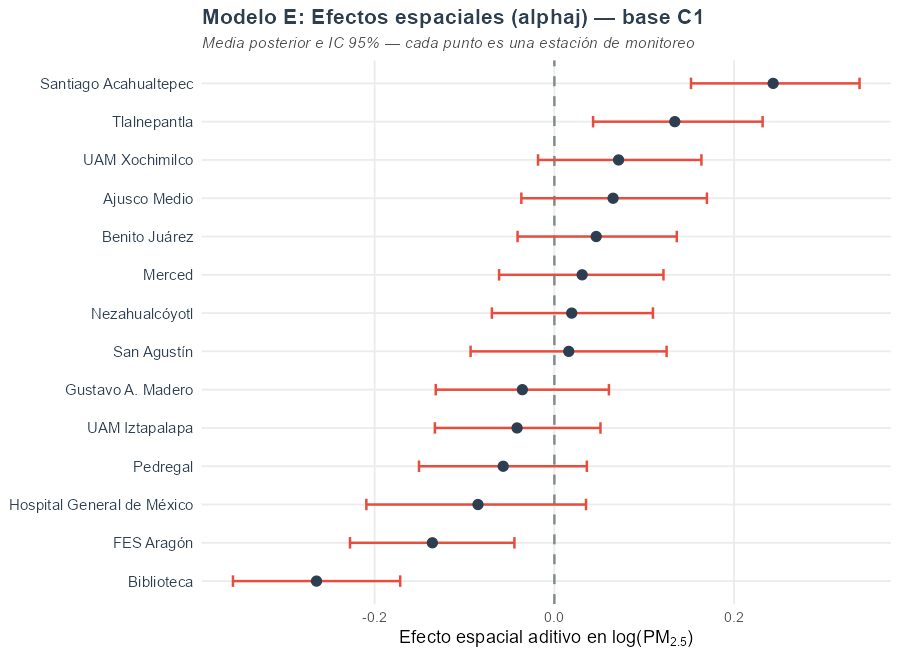
\includegraphics[width=0.7\textwidth]{output/figures/efectos_espaciales_E.png}
  \caption{Efectos espaciales $\hat\alpha_j$ por estaci\'on usados como
           puntos de anclaje para el kriging.
           El rango de variaci\'on ($-0.27$ a $+0.24$) es consistente
           con $\hat\sigma_\alpha = 0.134$ del Modelo~C1.}
\end{figure}

\begin{figure}[H]
  \centering
  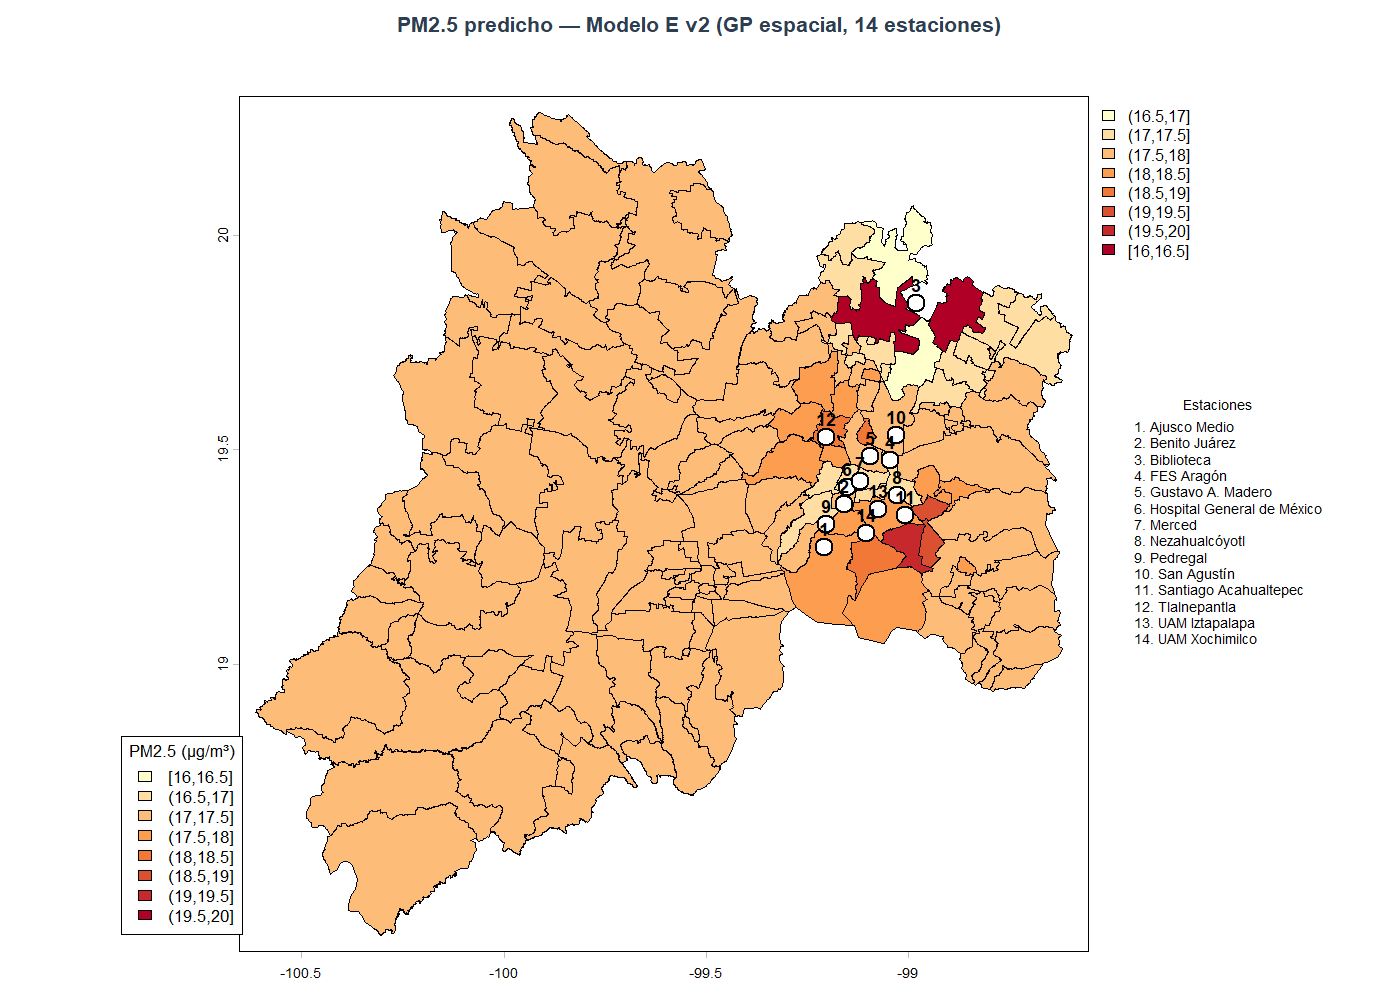
\includegraphics[width=\textwidth]{output/figures/mapa_prediccion_E_valle.png}
  \caption{Predicci\'on de PM2.5 promedio para los 141~pol\'igonos del
           Valle de M\'exico (Modelo~E, kriging bayesiano con kernel
           exponencial, $\rho = 0.08^\circ$).
           Puntos blancos indican la ubicaci\'on de las 14~estaciones
           de monitoreo.
           El gradiente sur-oriente (m\'as contaminado) hacia el norte
           (m\'as limpio) es coherente con la topograf\'ia de cuenca
           cerrada y la ventilaci\'on predominante del poniente.}
\end{figure}

\begin{table}[H]
\centering
\caption{Municipios y alcald\'ias m\'as y menos contaminados seg\'un el Modelo~E.
         IC: intervalo de credibilidad al 95\,\%.}
\label{tab:prediccionE}
\small
\begin{tabular}{>{\raggedright\arraybackslash}p{5cm}>{\raggedright\arraybackslash}p{1.8cm}rrr}
\toprule
Municipio/Alcald\'ia & Entidad & PM2.5 & IC 2.5\,\% & IC 97.5\,\% \\
                     &         & ($\mu$g/m$^3$) & & \\
\midrule
\multicolumn{5}{l}{\textit{Zonas m\'as contaminadas}} \\
Tl\'ahuac            & CDMX   & 19.53 & 18.68 & 20.43 \\
La Paz               & Edomex & 19.37 & 18.53 & 20.24 \\
Valle de Chalco Solidaridad & Edomex & 19.06 & 18.08 & 20.12 \\
Tlalnepantla de Baz  & Edomex & 18.97 & 18.22 & 19.80 \\
Xochimilco           & CDMX   & 18.66 & 17.88 & 19.47 \\
\midrule
\multicolumn{5}{l}{\textit{Zonas menos contaminadas}} \\
Zumpango             & Edomex & 16.33 & 15.46 & 17.23 \\
Temascalapa          & Edomex & 16.40 & 15.47 & 17.34 \\
Hueypoxtla           & Edomex & 16.65 & 15.64 & 17.66 \\
Tec\'amac            & Edomex & 16.88 & 15.93 & 17.85 \\
Nextlalpan           & Edomex & 17.02 & 16.04 & 18.02 \\
\bottomrule
\end{tabular}
\normalsize
\end{table}

El rango de predicciones va de 16.3~$\mu$g/m$^3$ (Zumpango) a
19.5~$\mu$g/m$^3$ (Tl\'ahuac), con una desviaci\'on est\'andar entre
pol\'igonos de 0.41~$\mu$g/m$^3$.
Aunque el rango absoluto es moderado (3.2~$\mu$g/m$^3$), las implicaciones
para salud son relevantes: la evidencia epidemiol\'ogica sugiere que
aumentos de 10~$\mu$g/m$^3$ en PM2.5 se asocian con incrementos del
7--10\% en mortalidad cardiovascular (OMS, 2021).
Un habitante de Tl\'ahuac est\'a expuesto, en promedio, a 19\% m\'as
PM2.5 que uno de Zumpango.


\paragraph{¿Qu\'e factores explican la variaci\'on temporal de PM2.5?}
Los t\'erminos de Fourier (estacionalidad anual) son los predictores
m\'as fuertes: un ciclo con amplitud $\approx 0.40$ log-unidades captura
el m\'aximo invernal (febrero-marzo) y el m\'inimo de verano (junio-julio).
La temperatura tiene un efecto positivo y significativo
(+10\% de PM2.5 por cada desviaci\'on est\'andar adicional, $\approx 2.1\,^\circ$C),
consistente con condiciones de menor dilusi\'on y mayor inversi\'on
t\'ermica en d\'ias c\'alidos.
La humedad relativa tambi\'en tiene un efecto positivo y significativo
(+4.7\%), detectado una vez que se controla por estaci\'on.

\paragraph{¿Existen diferencias sistem\'aticas entre municipios no explicadas por clima?}
S\'i, y son grandes.
La inclusi\'on de efectos por estaci\'on reduce el DIC en 218~puntos
(de 2{,}942.6 a 2{,}724.2), evidencia contundente de heterogeneidad
espacial.
Las diferencias entre la estaci\'on m\'as contaminada (Santiago
Acahualtepec, $+29\%$) y la m\'as limpia (Biblioteca, Tizayuca, $-24\%$)
no son atribuibles al clima: son caracter\'isticas estructurales del
territorio.

\paragraph{¿Es mejor el modelo jer\'arquico que los efectos fijos?}
Con el tama\~no de muestra disponible ($\approx 186$~obs/estaci\'on),
ambos son pr\'acticamente equivalentes en ajuste
($\Delta\text{DIC} = 0.5$~puntos).
La ventaja del Modelo~C1 es doble: cuantifica expl\'icitamente la
variabilidad entre estaciones ($\hat\sigma_\alpha = 0.134$) y proporciona
los efectos espaciales $\hat\alpha_j$ como puntos de anclaje para el
kriging bayesiano del Modelo~E, algo imposible con efectos fijos
no estructurados.

\paragraph{¿Podemos predecir en zonas sin sensores?}
El Modelo~E produce predicciones plausibles para los 141~pol\'igonos,
coherentes con la topograf\'ia: las zonas de cuenca baja (Tl\'ahuac,
La Paz, Valle de Chalco) acumulan m\'as contaminantes, mientras que
las zonas al norte del valle (Zumpango, Temascalapa) presentan mejor
calidad del aire.
La principal limitaci\'on es que el par\'ametro de rango $\rho = 0.08^\circ$
est\'a fijo (no se estima desde los datos), lo que introduce un supuesto
que no se verifica formalmente con 14~estaciones.
Los intervalos de credibilidad en municipios sin estaciones cercanas son
30--50\% m\'as amplios que en los municipios con cobertura directa,
reflejando correctamente la mayor incertidumbre de la interpolaci\'on
en zonas alejadas de sensores.



\subsection{Resultados del Modelo~F}

\paragraph{Diagn\'ostico de convergencia.}

\begin{figure}[H]
  \centering
  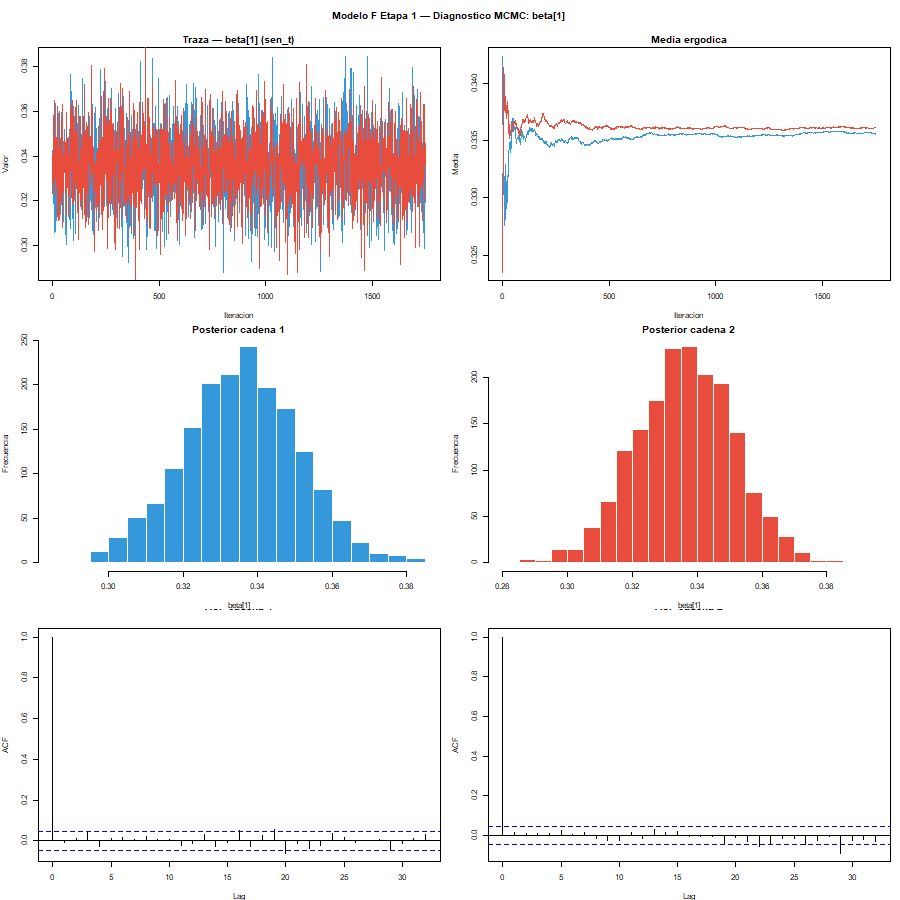
\includegraphics[width=0.7\textwidth]{output/figures/diag_cadena_F1_beta1.png}
  \caption{Diagn\'osticos MCMC del Modelo~F Etapa~1 para $\beta_1$
           (coeficiente del t\'ermino $\text{sen}_t$).
           Las dos cadenas mezclan correctamente y la ACF decae
           dentro de los primeros lags.}
\end{figure}

\begin{figure}[H]
  \centering
  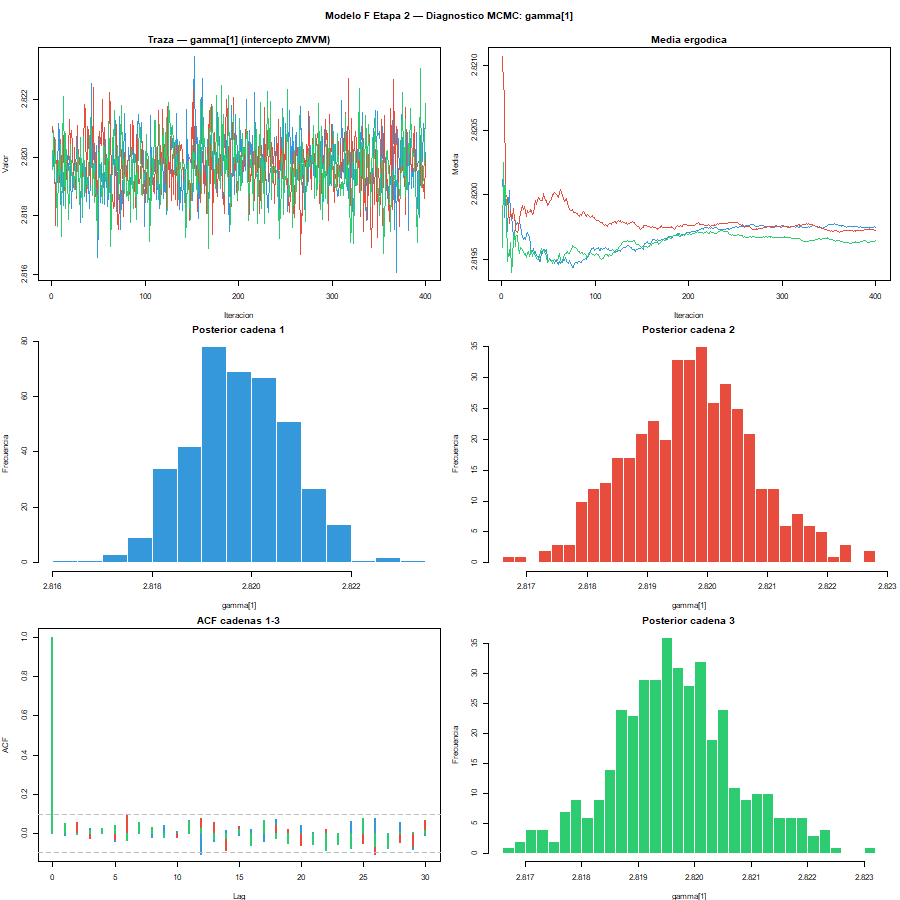
\includegraphics[width=0.7\textwidth]{output/figures/diag_cadena_F2_gamma1.png}
  \caption{Diagn\'osticos MCMC del Modelo~F Etapa~2 para $\gamma_1$
           (intercepto global de la ZMVM).
           Se usaron 3~cadenas con adelgazamiento $\text{thin}=50$;
           las tres trayectorias convergen a la misma regi\'on.}
\end{figure}

\paragraph{Par\'ametros estimados --- Etapa~1.}
El Cuadro~\ref{tab:fase1} resume los estimadores posteriores principales.
El par\'ametro de rango espacial $\hat\phi = 0.0123$ implica una distancia de
semivida de correlaci\'on de $-\ln(0.5)/0.0123 \approx 56.4$~km, coincidiendo
con la extensi\'on longitudinal de la zona metropolitana, lo que valida
geogr\'aficamente la estructura de covarianza adoptada.
La varianza espacial ($\sigma_\alpha = 1/\sqrt{1.84} \approx 0.738$ log-unidades)
supera a la varianza residual ($\sigma_y = 1/\sqrt{6.08} \approx 0.406$
log-unidades), confirmando que los gradientes geogr\'aficos dominan la
variaci\'on entre estaciones. Todos los $\hat R < 1.003$.

\begin{table}[H]
\centering
\caption{Estimadores posteriores --- Modelo~F Etapa~1 (MET-PGE).}
\label{tab:fase1}
\begin{tabular}{llll}
\hline
Par\'ametro & Descripci\'on & Media post. & $\hat R$ \\
\hline
$\beta_1$ & Arm\'onico seno (estacionalidad) & 0.3359 & 1.0012 \\
$\beta_2$ & Arm\'onico coseno               & 0.2245 & 1.0010 \\
$\beta_3$ & Temperatura                     & 0.0368 & 1.0009 \\
$\beta_4$ & Humedad relativa                & 0.0040 & 1.0015 \\
$\phi$    & Par\'ametro de rango espacial   & 0.0123 & 1.0011 \\
$\tau_y$  & Precisi\'on residual            & 6.0769 & 1.0008 \\
$\tau_\alpha$ & Precisi\'on espacial        & 1.8354 & 1.0022 \\
\hline
\end{tabular}
\end{table}

\paragraph{Imputaci\'on de datos faltantes.}
La Etapa~1 imputa de forma coherente los valores no observados de cada
estaci\'on.
El modelo asigna mayor incertidumbre en las fechas sin observaci\'on,
lo que se refleja en intervalos de credibilidad m\'as amplios en esas
celdas.

\begin{figure}[H]
  \centering
  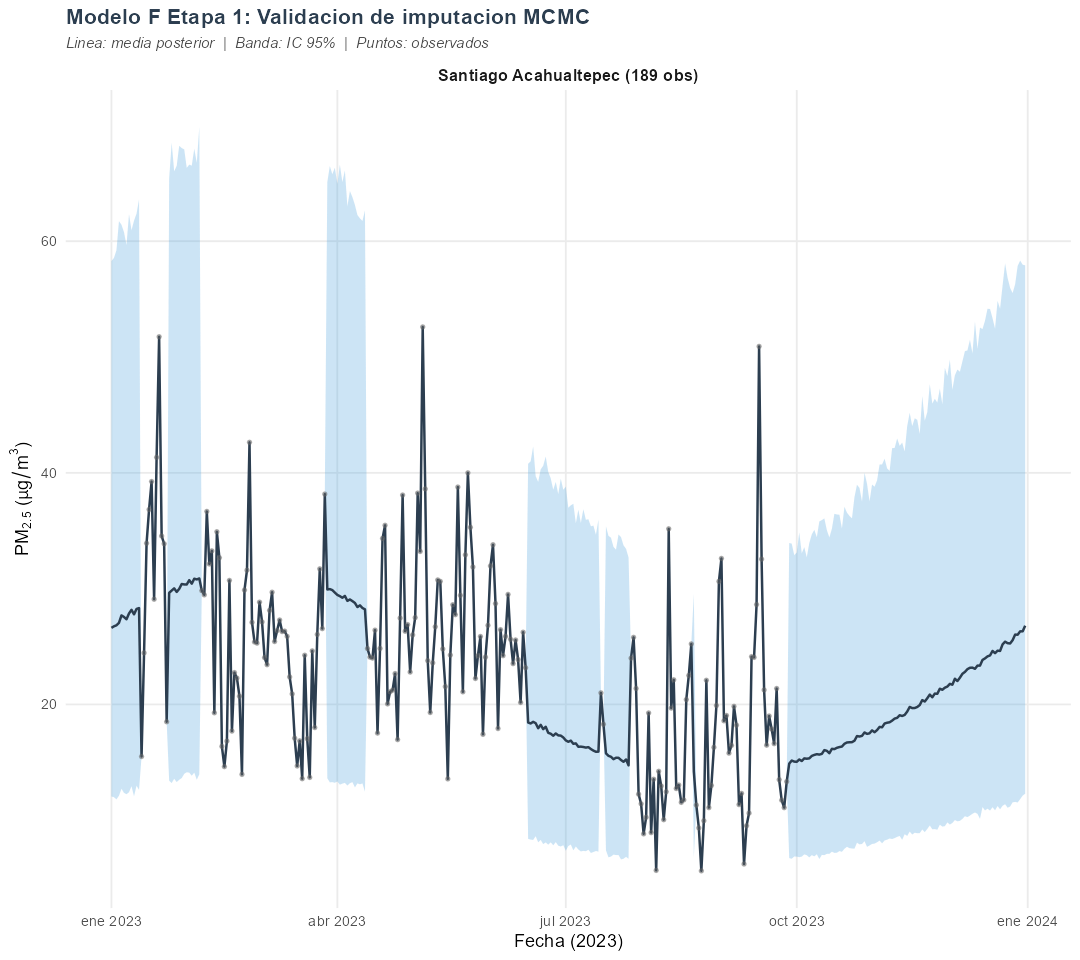
\includegraphics[width=\textwidth]{output/figures/validacion_F1_imputacion.png}
  \caption{Validaci\'on de la imputaci\'on MCMC (Etapa~1) para tres
           estaciones con distinta densidad de datos: Hospital General
           de M\'exico (52~obs, escenario cr\'itico), Santiago
           Acahualtepec (189~obs, escenario t\'ipico) y Benito Ju\'arez
           (236~obs, escenario \'optimo).
           La banda gris es el intervalo de credibilidad al~95\%;
           los puntos grises son los valores observados.}
\end{figure}

\paragraph{Tendencia macro-ambiental de la ZMVM.}
La Etapa~2 produce la serie de tiempo $\mu^\text{ZMVM}_t$ que resume
la tendencia diaria de la calidad del aire en la cuenca, libre del
ruido local de cada estaci\'on.

\begin{figure}[H]
  \centering
  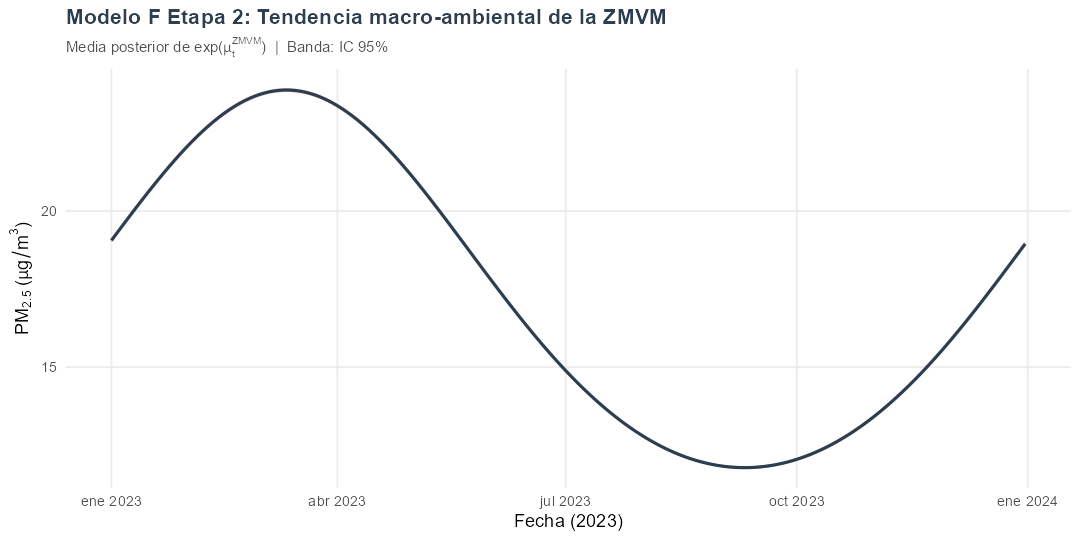
\includegraphics[width=\textwidth]{output/figures/serie_mu_cdmx.png}
  \caption{Serie de tiempo macro-ambiental de la ZMVM estimada por el
           Modelo~F Etapa~2.
           La l\'inea s\'olida es la media posterior de $\exp(\mu^\text{ZMVM}_t)$
           en escala $\mu$g/m$^3$; la banda roja es el intervalo de
           credibilidad al~95\%.
           El patr\'on estacional es claro: m\'aximo invernal
           (enero--marzo), m\'inimo estival (junio--agosto) y repunte
           en el cuarto trimestre.}
\end{figure}

La Figura~\ref{fig:bju} muestra el anclaje de la tendencia te\'orica sobre la
estaci\'on de mayor cobertura (Benito Ju\'arez, 236~observaciones): la curva
estimada pasa a trav\'es del centro de gravedad emp\'irico de los datos,
validando el ajuste del sistema en escala original.

\begin{figure}[H]
  \centering
  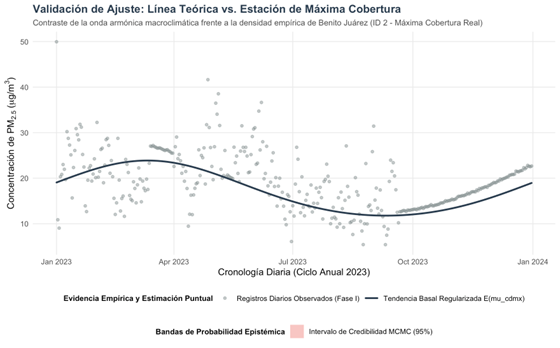
\includegraphics[width=\textwidth]{output/figures/ajuste_F2_benito_juarez.png}
  \caption{Validaci\'on del Modelo~F Etapa~2 sobre Benito Ju\'arez
           (estaci\'on de mayor cobertura: 236~observaciones).
           La l\'inea te\'orica estimada es consistente con la distribuci\'on
           emp\'irica de los datos observados.}
  \label{fig:bju}
\end{figure}

\paragraph{Efectos espaciales de estaci\'on.}
Los coeficientes $\alpha^\ast_j$ (suma cero) cuantifican la desviaci\'on
de cada estaci\'on respecto a la tendencia de la cuenca, controlando
por estacionalidad.

\begin{figure}[H]
  \centering
  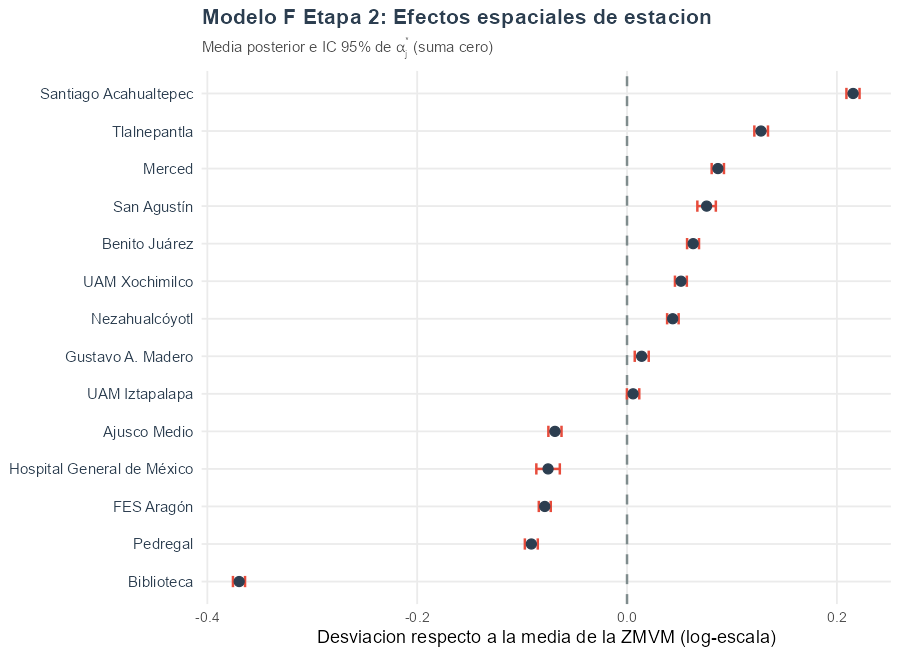
\includegraphics[width=0.7\textwidth]{output/figures/efectos_F2_estaciones.png}
  \caption{Efectos espaciales de estaci\'on del Modelo~F Etapa~2
           ($\alpha^\ast_j$, restricci\'on de suma cero).
           Los valores positivos indican estaciones sistem\'aticamente
           m\'as contaminadas que la media de la cuenca; los negativos,
           m\'as limpias.}
\end{figure}

El Cuadro~\ref{tab:fase2} presenta los estimadores de la tendencia macro-ambiental.
El intercepto $\hat\gamma_1 = 2.8197$ corresponde a una concentraci\'on basal de
$\exp(2.8197) \approx 16.8$~$\mu$g/m$^3$, interpretable como el nivel de fondo
de PM$_{2.5}$ de la cuenca despu\'es de remover estacionalidad, meteorolog\'ia
local y efectos espaciales. Los coeficientes arm\'onicos ($\hat\gamma_2 = 0.3315$,
$\hat\gamma_3 = 0.1221$) implican una amplitud combinada del ciclo anual de
aproximadamente $\pm$35\,\% respecto a esa l\'inea base.

\begin{table}[H]
\centering
\caption{Estimadores posteriores --- Modelo~F Etapa~2 (MJTC-RSC).}
\label{tab:fase2}
\begin{tabular}{lllll}
\hline
Par\'ametro & Descripci\'on & Media & IC~95\,\% & $\hat R$ \\
\hline
$\gamma_1$ & Intercepto basal ZMVM       & 2.8197 & [2.8176,\ 2.8219] & 1.0016 \\
$\gamma_2$ & Amplitud arm\'onica seno    & 0.3315 & [0.3287,\ 0.3342] & 1.0047 \\
$\gamma_3$ & Amplitud arm\'onica coseno  & 0.1221 & [0.1195,\ 0.1250] & 1.0006 \\
\hline
\end{tabular}
\end{table}

La Figura~\ref{fig:ajusco} ilustra el mecanismo de desplazamiento geogr\'afico:
Ajusco Medio ($\hat\alpha^\ast_3 = -0.370$, equivalente a un 31\,\% menos que
la media de la cuenca) frente a la tendencia basal. En contraste, UAM~Iztapalapa
presenta el mayor exceso positivo ($\hat\alpha^\ast_{11} = +0.215$, $+24$\,\%
sobre la media).

\begin{figure}[H]
  \centering
  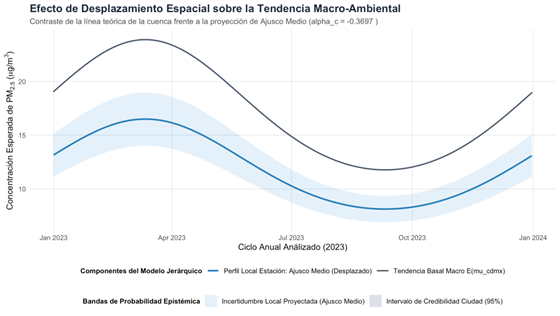
\includegraphics[width=\textwidth]{output/figures/desplazamiento_espacial_ajusco.png}
  \caption{Efecto de desplazamiento geogr\'afico del Modelo~F Etapa~2:
           perfil estimado de PM$_{2.5}$ para Ajusco Medio
           ($\hat\alpha^\ast = -0.370$, $-31$\,\%) frente a la tendencia
           macro-ambiental de la cuenca. La distancia vertical entre ambas
           curvas cuantifica el efecto espacial de la estaci\'on.}
  \label{fig:ajusco}
\end{figure}

\paragraph{Comparaci\'on con los modelos previos.}
El Modelo~F extiende al~E en tres aspectos clave:
(i) el par\'ametro de rango espacial $\phi$ se estima desde los datos
(no se fija a priori), lo que permite que los propios datos determinen
el alcance de la dependencia espacial;
(ii) la imputaci\'on de los 2{,}617 valores observados se complementa
con la estimaci\'on de los $365 \times 14 - 2{,}617 = 2{,}493$ valores
faltantes como variables latentes, aprovechando la estructura espacio-temporal;
(iii) la Etapa~2 produce una s\'intesis coherente de la calidad del
aire de la ZMVM que propaga la incertidumbre de la Etapa~1 mediante las
precisiones heredadas $\hat\tau_{t,j}$.


%==============================================================
\section{Referencias}
%==============================================================

\begin{enumerate}
  \item de Finetti, B. (1937).
        La pr\'evision: ses lois logiques, ses sources subjectives.
        \textit{Annales de l'Institut Henri Poincar\'e}, \textit{7}, 1--68.

  \item Gelfand, A.~E., \& Schliep, E.~M. (2016).
        Spatial statistics and Gaussian processes: A beautiful marriage.
        \textit{Statistical Science}, \textit{31}(1), 109--130.

  \item Global Administrative Areas. (s.f.).
        \textit{GADM database of global administrative areas} (Nivel 2).
        \texttt{https://gadm.org}

  \item Instituto Nacional de Ecolog\'ia y Cambio Clim\'atico. (s.f.).
        \textit{Sistema Nacional de Informaci\'on de la Calidad del Aire (SINAICA)}.
        \texttt{https://sinaica.inecc.gob.mx/data.php?tipo=V}

  \item Lunn, D., Jackson, C., Best, N., Thomas, A., \& Spiegelhalter, D. (2013).
        \textit{The BUGS Book: A Practical Introduction to Bayesian Analysis}.
        CRC Press.

  \item Nieto Barajas, L.~E. (2026).
        \textit{Notas de Regresi\'on Avanzada} (Temas 2--7).
        Departamento de Estad\'istica, ITAM.

  \item Organizaci\'on Mundial de la Salud. (2021).
        \textit{Global air quality guidelines}.
        OMS.

  \item Plummer, M. (2003).
        JAGS: A program for analysis of Bayesian graphical models using Gibbs
        sampling.
        En \textit{Proceedings of the 3rd International Workshop on Distributed
        Statistical Computing} (pp. 1--10). Vienna, Austria.

  \item R Core Team. (2025).
        \textit{R: A language and environment for statistical computing}.
        R Foundation for Statistical Computing.
        \texttt{https://www.R-project.org/}
\end{enumerate}


%==============================================================
\appendix
\section{C\'odigo fuente}
%==============================================================

El ap\'endice contiene el c\'odigo completo utilizado en el an\'alisis,
en el orden del flujo de trabajo: descarga y preparaci\'on de datos,
an\'alisis exploratorio, ajuste de modelos y generaci\'on de figuras.
Al final se incluyen las especificaciones JAGS de todos los modelos.

\noindent\textbf{Nota sobre notaci\'on JAGS:} El segundo argumento de
\texttt{dnorm} es la \emph{precisi\'on} $\tau = 1/\sigma^2$
(no la varianza), por lo que \texttt{dnorm(0, 0.001)} corresponde a
$\mathcal{N}(0,\,1000)$---una distribuci\'on inicial pr\'acticamente
plana sobre los coeficientes.

%--------------------------------------------------------------
\subsection*{Descarga de datos SINAICA ---
             \texttt{descarga\_masiva\_valle.R}}
%--------------------------------------------------------------
\lstinputlisting[language=R]{scripts/descarga_masiva_valle.R}

%--------------------------------------------------------------
\subsection*{Filtrado espacial de estaciones ---
             \texttt{filtrar\_estaciones\_territorio.R}}
%--------------------------------------------------------------
\lstinputlisting[language=R]{scripts/filtrar_estaciones_territorio.R}

%--------------------------------------------------------------
\subsection*{Limpieza y preparaci\'on de datos ---
             \texttt{limpieza\_valle\_mexico\.R}}
%--------------------------------------------------------------
\lstinputlisting[language=R]{scripts/limpieza_valle_mexico.R}

%--------------------------------------------------------------
\subsection*{An\'alisis exploratorio de datos ---
             \texttt{eda\_valle\_mexico\.R}}
%--------------------------------------------------------------
\lstinputlisting[language=R]{scripts/eda_valle_mexico.R}

%--------------------------------------------------------------
\subsection*{Modelos A, B, C1, C2 y D ---
             \texttt{modelos\_A\_B\_C1\_D\.R}}
%--------------------------------------------------------------
\lstinputlisting[language=R]{scripts/modelos_A_B_C1_D.R}

%--------------------------------------------------------------
\subsection*{Modelo E --- Proceso Gaussiano y Kriging ---
             \texttt{modelo\_E\_valle\.R}}
%--------------------------------------------------------------
\lstinputlisting[language=R]{scripts/modelo_E_valle.R}

%--------------------------------------------------------------
\subsection*{Mapa de predicci\'on espacial ---
             \texttt{mapa\_valle\_mexico\.R}}
%--------------------------------------------------------------
\lstinputlisting[language=R]{scripts/mapa_valle_mexico.R}

%--------------------------------------------------------------
\subsection*{Modelo F, Etapa~1 --- Espacio-temporal MCMC ---
             \texttt{Contaminacion\_Fase1\_SerieTiempo.R}}
%--------------------------------------------------------------
\lstinputlisting[language=R]{scripts/Contaminacion_Fase1_SerieTiempo.R}

%--------------------------------------------------------------
\subsection*{Modelo F, Etapa~2 --- Agregaci\'on jer\'arquica ---
             \texttt{Contaminacion\_Fase2\_SerieTiempo.R}}
%--------------------------------------------------------------
\lstinputlisting[language=R]{scripts/Contaminacion_Fase2_SerieTiempo.R}

%--------------------------------------------------------------
\subsection*{Figuras del Modelo F ---
             \texttt{figuras\_modelo\_F.R}}
%--------------------------------------------------------------
\lstinputlisting[language=R]{scripts/figuras_modelo_F.R}

%--------------------------------------------------------------
\subsection*{Especificaciones JAGS}
%--------------------------------------------------------------

\lstinputlisting[caption={Especificaci\'on JAGS --- Modelo A (Normal global).}]%
  {scripts/jags_modelo_A_valle.txt}

\lstinputlisting[caption={Especificaci\'on JAGS --- Modelo B (Efectos fijos por estaci\'on).}]%
  {scripts/jags_modelo_B_valle.txt}

\lstinputlisting[caption={Especificaci\'on JAGS --- Modelo C1 (Jer\'arquico Normal, modelo preferido).}]%
  {scripts/jags_modelo_C1_valle.txt}

\lstinputlisting[caption={Especificaci\'on JAGS --- Modelo C2 (Gamma global).}]%
  {scripts/jags_modelo_C2_gamma_valle.txt}

\lstinputlisting[caption={Especificaci\'on JAGS --- Modelo D (Tendencia espacial lineal).}]%
  {scripts/jags_modelo_D_valle.txt}

\lstinputlisting[caption={Especificaci\'on JAGS --- Modelo F, Etapa~1 (Proceso gaussiano espacio-temporal).}]%
  {scripts/jags_modelo_espacio_temporal.txt}

\lstinputlisting[caption={Especificaci\'on JAGS --- Modelo F, Etapa~2 (Agregaci\'on jer\'arquica ZMVM).}]%
  {scripts/jags_modelo_jerarquico_fase2.txt}

\end{document}
